%\RequirePackage[l2tabu,orthodox]{nag}

% TODO: decide if one-sided/two-sided
%\documentclass[headsepline,footsepline,footinclude=false,fontsize=11pt,paper=a4,listof=totoc,bibliography=totoc,BCOR=12mm,DIV=12]{scrbook} % two-sided % original source stated: BCOR=12mm,DIV=12
\documentclass[10pt,b5paper,twoside,openright, headsepline, footsepline, footinclude=false,oneside,fontsize=11pt,paper=b5,listof=totoc,bibliography=totoc,DIV=12]{book} % one-sided
% TODO: change citation style in settings
\PassOptionsToPackage{table,svgnames,dvipsnames,xcdraw}{xcolor}

\usepackage[utf8]{inputenc}
\usepackage[T1]{fontenc}
\usepackage[sc]{mathpazo}
\usepackage[ngerman,english,norsk]{babel} % english is the same as american or USenglish
\usepackage[autostyle]{csquotes}
\usepackage{adjustbox} %rotating tables
\usepackage{rotating,tabularx}
\usepackage[table,xcdraw]{xcolor}
\usepackage[%
  backend=biber,
  url=true,
  style=numeric, % alphabetic, numeric
  sorting=none, % default == nty, https://tex.stackexchange.com/questions/51434/biblatex-citation-order
  maxnames=4,
  minnames=3,
  maxbibnames=99,
  giveninits,
  uniquename=init]{biblatex} % TODO: adapt citation style
\usepackage{graphicx}
\usepackage{color}
\usepackage{mathtools}
\usepackage{scrhack} % necessary for listings package
\usepackage{listings}
\usepackage{lstautogobble}
\usepackage{placeins}
%\usepackage{subcaption}

\usepackage{subfig}
\captionsetup{compatibility=false}
\usepackage{tikz}
\usepackage{pgfplots}
\usepackage{pgfplotstable}
\usepackage{booktabs} % for better looking table creations, but bad with vertical lines by design (package creator despises vertical lines)
\usepackage[final]{microtype}
\usepackage{caption}
\usepackage[hidelinks]{hyperref} % hidelinks removes colored boxes around references and links
\usepackage{ifthen} % for comparison of the current language and changing of the thesis layout
\usepackage{pdftexcmds} % string compare to work with all engines
\usepackage{paralist} % for condensed enumerations or lists
 % for having figures side by side
\usepackage{siunitx} % for physical accurate units and other numerical presentations
\usepackage{multirow} % makes it possible to have bigger cells over multiple rows in a table
\usepackage{array} % different options for table cell orientation
\usepackage{makecell} % allows nice manual configuration of cells with linebreaks in \thead and \makecell with alignments
\usepackage{pdfpages} % for including multiple pages of pdfs
\usepackage{adjustbox} % can center content wider than the \textwidth
\usepackage{tablefootnote} % for footnotes in tables as \tablefootnote
\usepackage{threeparttable} % another way to add footnotes as \tablenotes with \item [x] <your footnote> after setting \tnote{x} 

\usepackage{soul} % For highlighting text

\usepackage{amsmath}

\usepackage{nomencl} % Nomenclature
\usepackage{etoolbox}


\usepackage{booktabs}
\usepackage{multirow}

\usepackage{hyperref}
\hypersetup{
    colorlinks=true,
    linkcolor=blue,
    filecolor=magenta,      
    urlcolor=blue,
}
 
\urlstyle{same}

% https://tex.stackexchange.com/questions/42619/x-mark-to-match-checkmark
\usepackage{amssymb}% http://ctan.org/pkg/amssymb
%\usepackage{pifont}% http://ctan.org/pkg/pifont
%\newcommand{\cmark}{\ding{51}}%
%\newcommand{\xmark}{\ding{55}}%

\usepackage{caption}
%\usepackage{subcaption}

\usepackage[acronym,xindy,toc]{glossaries} % TODO: include "acronym" if glossary and acronym should be separated
\makeglossaries
\loadglsentries{pages/glossary.tex} % important update for glossaries, before document


\bibliography{bibliography}

%\setkomafont{disposition}{\normalfont\bfseries} % use serif font for headings
\linespread{1.5} % adjust line spread for mathpazo font

% Add table of contents to PDF bookmarks
\BeforeTOCHead[toc]{{\cleardoublepage\pdfbookmark[0]{\contentsname}{toc}}}


% Settings for pgfplots
%\pgfplotsset{compat=newest}
%\pgfplotsset{
  % For available color names, see http://www.latextemplates.com/svgnames-colors
  %cycle list={TUMBlue\\TUMAccentOrange\\TUMAccentGreen\\TUMSecondaryBlue2\\TUMDarkGray\\},
%}

% Settings for lstlistings

% Use this for basic highlighting
\lstset{%
  basicstyle=\ttfamily,
  columns=fullflexible,
  autogobble,
  keywordstyle=\bfseries\color{TUMBlue},
  stringstyle=\color{TUMAccentGreen}
}

% use this for C# highlighting
 %\setmonofont{Consolas} %to be used with XeLaTeX or LuaLaTeX
 \definecolor{bluekeywords}{rgb}{0,0,1}
 \definecolor{greencomments}{rgb}{0,0.5,0}
 \definecolor{redstrings}{rgb}{0.64,0.08,0.08}
 \definecolor{xmlcomments}{rgb}{0.5,0.5,0.5}
 \definecolor{types}{rgb}{0.17,0.57,0.68}


% Settings for search order of pictures
\graphicspath{
    {logos/}
    {figures/}
}

% Set up hyphenation rules for the language package when mistakes happen
\babelhyphenation[english]{
an-oth-er
ex-am-ple
}

% Decide between
%\newcommand{\todo}[1]{\textbf{\textsc{\textcolor{TUMAccentOrange}{(TODO: #1)}}}} % for one paragraph, otherwise error!
%\newcommand{\done}[1]{\textit{\textsc{\textcolor{TUMAccentBlue}{(Done: #1)}}}} % for one paragraph, otherwise error!
% and
%\newcommand{\todo}[1]{{\bfseries{\scshape{\color{TUMAccentOrange}[(TODO: #1)]}}}} % for multiple paragraphs
\newcommand{\done}[1]{{\itshape{\scshape{\color{TUMAccentBlue}[(Done: #1)]}}}} % for multiple paragraphs
% for error handling of intended behavior in your latex documents.

\newcommand{\tabitem}{~~\llap{\textbullet}~~}

\newcolumntype{P}[1]{>{\centering\arraybackslash}p{#1}} % for horizontal alignment with limited column width
\newcolumntype{M}[1]{>{\centering\arraybackslash}m{#1}} % for horizontal and vertical alignment with limited column width
\newcolumntype{L}[1]{>{\raggedright\arraybackslash}m{#1}} % for vertical alignment left with limited column width
\newcolumntype{R}[1]{>{\raggedleft\arraybackslash}m{#1}} % for vertical alignment right with limited column width

% Math equation font sizes
\usepackage{environ}
\NewEnviron{NORMAL}{%
    \scalebox{1.1}{$\BODY$}
}
\NewEnviron{HUGE}{%
    \scalebox{1.3}{$\BODY$}
}
\NewEnviron{SMALL}{%
    \scalebox{0.7}{$\BODY$}
}

% Math norm
\usepackage{commath}


\usepackage{xcolor}
 

\definecolor{codegreen}{rgb}{0,0.6,0}
\definecolor{codegray}{rgb}{0.5,0.5,0.5}
\definecolor{codepurple}{rgb}{0.58,0,0.82}
\definecolor{backcolour}{rgb}{0.95,0.95,0.92}
\usepackage{color} %red, green, blue, yellow, cyan, magenta, black, white
\definecolor{mygreen}{RGB}{28,172,0} % color values Red, Green, Blue
\definecolor{mylilas}{RGB}{170,55,241}

% ``listings'' package settings
\definecolor{dkgreen}{rgb}{0,0.6,0}
\definecolor{gray}{rgb}{0.5,0.5,0.5}
\definecolor{pink}{rgb}{0.63, 0.13, 0.94}


\lstset{language=Matlab, 
	keywords={break, case, catch, continue, else, elseif, end, for, function,
		global, if, otherwise, persistent, return, switch, try, while},
	basicstyle=\footnotesize, % scriptsize for mindre
	keywordstyle=\color{blue},
	commentstyle=\color{dkgreen},
	stringstyle=\color{pink},
	numbers=left,
	numberstyle=\tiny\color{gray},
	stepnumber=1,
	numbersep=10pt,
	backgroundcolor=\color{white},
	tabsize=4,
	showspaces=false,
	frame = single, 
    showstringspaces=false}


% TODO: change thesis information
\newcommand*{\getUniversity}{Norwegian University of Science and Technology}
\newcommand*{\getFaculty}{Department of Engineering Cybernetics}
\newcommand*{\getTitle}{Simulator for Obstacle Aided Locomotion in Snake Robots}
\newcommand*{\getAuthor}{Atussa Koushan}
\newcommand*{\getDoctype}{Specialization Project Report}
%\newcommand*{\getSupervisor}{Supervisor}
%\newcommand*{\getAdvisor}{Advisor}
\newcommand*{\getSubmissionDate}{December 17th 2019}
%\newcommand*{\getSubmissionLocation}{Munich}

%--------- Code Highlighting Style
\usepackage[utf8]{inputenc}

\usepackage{listings}
\usepackage{color}
 

%---------

\makenomenclature

\begin{document}

% TODO: decide on used language
%\selectlanguage{ngerman}
\selectlanguage{english}

% Set page numbering to avoid "destination with the same identifier has been already used" warning for cover page.
% (see https://en.wikibooks.org/wiki/LaTeX/Hyperlinks#Problems_with_Links_and_Pages).
\pagenumbering{alph}


\frontmatter{}

\begin{titlepage}
  \centering

  \IfFileExists{logos/ntnulogo.pdf}{%
    
\includegraphics[height=13mm]{logos/ntnulogo.pdf}
  }{%
    \vspace*{20mm}
  }

  \vspace{5mm}
  {\large\MakeUppercase{\getUniversity{}}}\\

  \vspace{10mm}
  {\large\MakeUppercase{\getFaculty{}}}\\
  \vspace{3mm}



  \vspace{20mm}
  {\Large \getDoctype{}}

  \makeatletter
  \vspace{15mm}
  \ifthenelse{\pdf@strcmp{\languagename}{english}=0}
  {



  \vspace{10mm}
  {\huge\bfseries \foreignlanguage{english}{\getTitle{}}}
  }
  \makeatother

 \vspace{15mm}
  \begin{tabular}{l l}
    Author:          & \getAuthor{} \\
    %Advisor:         & \getAdvisor{} \\
    Submission Date: & \getSubmissionDate{} \\
  \end{tabular}

\end{titlepage}

%\input{pages/disclaimer}
%\input{pages/acknowledgements} % TODO: if you don't have anyone to thank for or don't wish to publish it, comment this line out.
\chapter{\abstractname}

%TODO: Abstract

%A number of different principles for snake robot locomotion have been proposed and tested, many of which are based on heuristic rules and stiff position controlled joints. A more physics-based and compliant method is being developed which is based on the formalism of hybrid position/force control. In this assignment you will study this emerging technique and simulate an idealized two-dimensional snake robot propelled by contact forces based on hybrid position/force control in an idealized environment comprising frictionless movement and extentionless environmental assets (“obstacles”).\\


Snake robots are robust serial link robots able to propel themselves through uneven and irregular terrain. As opposed to traditional mobile robots, the snake robot can utilize obstacles found in the environment to push itself forward along a predefined path. The aforementioned mode of locomotion is referred to as \textbf{obstacle aided locomotion (OAL)}. The challenge of both controlling the shape and contact forces of the snake robot has motivated the study of \textbf{hybrid position/force control (HPFC)}, with special emphasis on application within OAL.

%\textbf{Obstacle aided locomotion (OAL)} is a mode of snake robot locomotion in which obstacles are utilized for propulsion, rather than avoided. 



The main principle of HPFC together with a simplified 2-dimensional model of the snake robot and its environment are the backbone of the developed MATLAB simulator. The objective of this simulator is to visualize the behavior of the snake robot and OAL in simple path following scenarios.

%\textbf{Hybrid position/force control (HPFC)} is studied with emphasis on application within OAL and general simultaneous contact force- and shape control of snake robots. The main principle of HPFC together with a simplified model of the snake robot and its environment are the backbone of the developed MATLAB simulator. The objective of this simulator is visualization of the snake robots behavior and OAL in simple path following cases.

Relevant experiments conducted during this study has proven the simulator to be a great resource for presenting concepts and study limitations and possibilities within OAL. However, a geometrical approximation was made to the applied part of the HPFC concept during development of the simulator, which has led to some deviations from the true dynamics of the system. The code of the simulation program can be provided upon request.


\makeatletter
\ifthenelse{\pdf@strcmp{\languagename}{english}=0}


\makeatother



%TODO: Abstract in other language





\chapter{Sammendrag}

%Snake robots are robust serial link robots able to propel uneven and irregular terrain. As opposed to traditional mobile robots, the snake robot can utilize the obstacles found in the environment to push itself forward along a predefined path. The aforementioned mode of locomotion is referred to as \textbf{obstacle aided locomotion (OAL)}. The challenge of both controlling the shape and contact forces of the snake robot has motivated the study of \textbf{hybrid position/force control (HPFC)}, with special emphasis on application within OAL.

%The main principle of HPFC together with a simplified 2-dimensional model of the snake robot and its environment are the backbone of the developed MATLAB simulator. The objective of this simulator is to visualize the snake robots behavior and OAL in simple path following scenarios.

%From relevant experiments, the simulator has proven to be a great resource for presenting concepts and study limitations and possibilities within OAL. However, a geometrical approximation was made to the applied part of the HPFC concept during development of the simulator, which has led to some deviations from the true dynamics of the system. The code of the simulation program can be provided upon request.

Slangeroboter er robuste seriekoblede roboter som evner å traversere ujevne og uregelmessige terreng. I motsetning til tradisjonelle mobile roboter, kan slangeroboter utnytte hindringer i miljøet sitt ved å dytte seg selv fram langs en forhåndsdefinert bane. Denne bevegelsesarten blir omtalt som \textbf{obstacle aided locomotion (OAL)} eller hindringsbasert fremdrift. Utfordringen som trer fram ved kontrollering av både formen og kontaktkreftene til slangeroboten har motivert studiet av  \textbf{hybrid position/force control (HPFC)} eller hybrid posisjons- og kraftstyring, med spesiell vekt på applikasjoner innenfor OAL.

Hovedprinsippet bak HPFC kombinert med en todimensjonal modell av slangen og dens miljø er selve fundamentet til den utviklede MATLAB-simulatoren. Formålet med denne simulatoren er å visualisere slangerobotens oppførsel og OAL i enkle banefølgingsscenarioer.

Simulatoren har fra relevante eksperimenter utført under studiet vist seg å være et godt verktøy for presentering av konsepter og studere både begrensninger og muligheter knyttet til OAL. På en annen side har en geometrisk approksimasjon av den anvendte delen av HPFC i simulatoren ført til noen avvik fra den sanne dynamikken i systemet. Koden for simuleringsprogrammet er til disposisjon ved ønske.

\makeatletter
\ifthenelse{\pdf@strcmp{\languagename}{english}=0}


\makeatother



%TODO: Abstract in other language





\chapter{Preface}

This report covers the work of the specialization project for the masters study Cybernetics and Robotics at the Norwegian University of Science and Technology (NTNU). 
The work has been conducted with great counselling from supervisor Øyvind Stavdahl. A lot of Stavdahl's previous work and notes also make out the mathematical foundation of the project. 

The developed snake robot simulator is based in MATLAB. The package \textit{Symbolic Math Toolbox} has been actively used. All code is written by me and can be accessed through the github repository blablalba.

The figures presented throughout the report are designed by me, unless stated otherwise.

\medskip
\begin {flushright}
  \textit{Atussa Koushan} \\
  \textsc {17.12.2019} \\
  Trondheim, Norway
\end {flushright}



\makeatletter
\ifthenelse{\pdf@strcmp{\languagename}{english}=0}


\makeatother





%\renewcommand{\nomname}{List of Symbols}

%\renewcommand*{\nompreamble}{\footnotesize}

\renewcommand\nomgroup[1]{%
    \footnotesize
  \item[\bfseries
  \ifstrequal{#1}{R}{\small Robot kinematics symbols}{%
  \ifstrequal{#1}{D}{\small Robot dynamics symbols}{%
  \ifstrequal{#1}{C}{\small Control symbols}{%
  \ifstrequal{#1}{S}{\small Spaces}{%
  \ifstrequal{#1}{A}{\small Abbreviations}{}}}}}%
]}


\renewcommand{\nompreamble}{The following list describes several symbols and abbreviations used in the report. All units follow the SI unit system.}

%---------------------------------------------------------------------------------
%%-------------------------------- KINEMATICS ------------------------------------
%---------------------------------------------------------------------------------

\nomenclature[R, 01]{$n$}{Number of links}
\nomenclature[R, 02]{$N$}{Number of generalized coordinates}
\nomenclature[R, 03]{$m$}{Link mass}
\nomenclature[R, 04]{$l$}{Link length}

\nomenclature[R, 05]{$\mathbf{q}$}{Generalized coordinates}
\nomenclature[R, 06]{$\phi_i$}{Joint angle of link $i$}

\nomenclature[R, 10]{$(x_0, y_0)$}{Position of tail in base frame}
\nomenclature[R, 11]{$(x_i, y_i)$}{Position of endpoint of link $i$ in base frame $b$}
\nomenclature[R, 12]{$(x_{c,i}, y_{c,i})$}{Position of contact point on link $i$ in base frame $b$}
\nomenclature[R, 13]{$d_{c,i}$}{Distance from joint $i$ to contact point on link $i$}
\nomenclature[R, 14]{$\mathbf{T_{bi}}$}{Transformation matrix from base frame to frame of link $i$}
\nomenclature[R, 15]{$\mathbf{T_{bci}}$}{Transformation matrix from base frame to frame of contact point on link $i$}
\nomenclature[R, 16]{$\mathbf{v_i}$}{Velocity of endpoint of link $i$ in base frame $b$}
\nomenclature[R, 17]{$\mathbf{v_{c,i}}$}{Velocity of contact point on link $i$ in base frame $b$}

\nomenclature[R, 18]{$\mathbf{J}$}{Jacobian matrix}
\nomenclature[R, 19]{$\mathbf{J_c}$}{Jacobian matrix for contact point}

\nomenclature[R, 20]{$\theta$}{Joint angle deviation from path}
\nomenclature[R, 21]{$r_{safety}$}{Radius around obstacle}

%---------------------------------------------------------------------------------
%%-------------------------------- DYNAMICS --------------------------------------
%---------------------------------------------------------------------------------

\nomenclature[D, 01]{$\boldsymbol{\tau}$}{Generalized torques}
\nomenclature[D, 02]{$\boldsymbol{\tau}_m$}{Joint motor torques}
\nomenclature[D, 03]{$\boldsymbol{\tau}_c$}{Joint torques from external forces}

\nomenclature[D, 04]{$\mathbf{M}$}{Mass matrix}
\nomenclature[D, 05]{$\mathbf{C}$}{Coriolis matrix}
\nomenclature[D, 06]{$\mathbf{g}$}{Gravity matrix}

\nomenclature[D, 07]{$L$}{Lagrangian}
\nomenclature[D, 08]{$K, P$}{Kinetic and potential energy}
\nomenclature[D, 09]{$I$}{Moment of inertia of rod}

\nomenclature[D, 10]{$\mathbf{f}^b_{c,i}, \mathbf{f}^i_{c,i}$}{External force on link $i$ in base frame and frame of link $i$}
\nomenclature[D, 11]{$\alpha_i$}{Angle of link $i$ relative to base frame}

\nomenclature[D, 12]{$\mathbf{r}$}{End effector position in the base frame $b$}
\nomenclature[D, 13]{$p(\mathbf{r})$}{Constraint hypersurface}
\nomenclature[D, 14]{$\mathbf{E_F}$}{Matrix of hypersurface unit normal vectors}
\nomenclature[D, 15]{$\mathbf{f}^b$}{End effector force on hypersurface}

\nomenclature[D, 16]{$\mathbf{p}$}{Momentum}

%---------------------------------------------------------------------------------
%%-------------------------------- CONTROL ---------------------------------------
%---------------------------------------------------------------------------------

\nomenclature[C, 01]{$K_p$}{Proportional gain}
\nomenclature[C, 02]{$K_d$}{Derivative gain}
\nomenclature[C, 03]{$\zeta$}{Damping ratio}
\nomenclature[C, 04]{$\omega_n$}{Natural frequency}
\nomenclature[C, 05]{$\mathbf{q_d}$}{Desired joint angles}
\nomenclature[C, 06]{$\mathbf{q_e}$}{Joint angle errors}

%---------------------------------------------------------------------------------
%%-------------------------------- SPACES ----------------------------------------
%---------------------------------------------------------------------------------

\nomenclature[S, 01]{$\mathbb{T}$}{Task space}
\nomenclature[S, 02]{$\mathbb{F}$}{Force space}
\nomenclature[S, 03]{$\mathbb{M}$}{Motion space}
\nomenclature[S, 04]{$\mathbb{C}$}{Constraint space}
\nomenclature[S, 05]{$\mathbb{P}$}{Propulsion space}
\nomenclature[S, 06]{$\mathbb{S}$}{Shape space}

%---------------------------------------------------------------------------------
%%-------------------------------- ABBREVIATIONS ---------------------------------
%---------------------------------------------------------------------------------

\nomenclature[A, 01]{HPFC}{Hybrid Position/Force Control}
\nomenclature[A, 02]{OAL}{Obstacle Aided Locomotion}
\nomenclature[A, 03]{HOAL}{Hybrid Obstacle Aided Locomotion}


\microtypesetup{protrusion=false}
\tableofcontents{}
\printnomenclature

\listoffigures{}
\listoftables{}
\microtypesetup{protrusion=true}


\mainmatter{}


% Chapters
% !TeX root = ../main.tex
% Add the above to each Chapter to make compiling the PDF easier in some editors.

\chapter{Introduction}\label{Chapter:introduction}

\section{Previous work}
The department of engineering cybernetics at the Norwegian University of Science and Technology (NTNU) has made significant contributions to the field of snake robot control, related to both aquatic snake-like propulsion and efficient snake robot locomotion on flat surfaces \cite{StavdahlNote}.

However, snakes can also utilize irregularities in a terrain. Consequently, Transeth et al. \cite{transeth2008snake} suggested the term \textit{Obstacle Aided Locomotion (OAL)} for snake robots that actively use walls or external objects for means of propulsion.

A relevant concept for attainment of this type of propulsion is \textit{Hybrid Position/Force Control (HPFC)}. The concept was first introduced by Raibert and Craig et al. in 1981 \cite{raibert1981hybrid}. West and Asada \cite{west1985method} further proposed a method for the design of HPFC controllers in 1985 for constrained manipulators that are in contact with the environment at multiple points. This method aims at controlling the position and force at the manipulator joints with kinematics-based projections such that the motion at the end effector, and the force at the contacts with the environment are those required for performing the task. Yoshikawa \cite{yoshikawa1987dynamic} advanced the constraint analysis by taking the dynamics into consideration.


Stavdahl \cite{StavdahlNote} proposed the combination of OAL and HPFC, leading to the term \textit{Hybrid Obstacle Aided Locomotion (HOAL)}. It is still a small area of research, but has a lot of potential in the area of e.g. rescue robots in cluttered environments. Klafstad \cite{TorjusOppg} later summarized the concept of HPFC in snake robots with special emphasis on the method of West and Asada \cite{west1985method}.

\section{Scope of the project}
The goal of this project is to establish a suitable and simplified 2-dimensional model of the idealized robot and its environment. A simulator is then to be developed from scratch based on this model and the concepts of OAL and HPFC. The purpose of the simulator is from the project task interpreted to be a platform for showing the aforementioned concepts on snake robots, rather than data generation for physical purposes.
Seeing as HOAL still is a fresh area of research and has little solid theoretical backdrop, this work goes in the direction of a proof-of-concept and experiments were performed to verify the method.

\subsection{Simplifications}
Due to the strict time constraints of the project and somewhat vague outlines, simplifications have been made to provide for a specific end goal. The simulator is restricted to handle bounded and well-defined scenarios with slow dynamics. Furthermore, the calculation of interaction forces in the simulator is neglected in favor of an easier discrete projection method that only takes joint velocities into consideration. This geometrical approximation is explained in further detail in Chapter \ref{ch:simulator} and discussed in Chapter \ref{ch:discussion}. The simplifications have led to some deviations from the true dynamical behavior of the robot when it is in contact with obstacles. As the velocity is changed without regard to energy conservation, this is most prominent in cases where the velocity is increased rather than decreased.

All assumptions regarding the employed model can be found in Chapter \ref{ch:model_specs}.

\subsection{Contributions}
A lot of the contributions connected to the limited research environment of HOAL have been clarification of the associated formulations and theoretical aspects.
Additionally, specific contributions are 

\begin{itemize}
    \item Study and analysis of HPFC, both with and without a dynamics consideration.
    \item Develpoment of a mathematical model of the snake robot and its environment           related to the given problem formulation.
    \item MATLAB simulator for demonstration of simple and germane HOAL-scenarios.
        It should be noted that this simulator is programmed from scratch and made in the context of an experimental study.
        On the basis of the generalized structure of the simulator program, several of the related modules can be applied to future implementations.
    \item Testing of the simulator performance and an evaluation of the associated             limitations.
    \item Evaluation of the OAL concept and discussion of remaining challenges, as well     as proposals for improvement.
\end{itemize}

\section{Report structure}
It is assumed that the reader is familiar with basic robotics and control theory. Please see \cite{lynch2017modern}, \cite{lynch2017modernCompTorque}, \cite{waldron2016kinematics}, \cite{liljeback2012snake} for a more thorough explanation of the topics.

The report first introduces the specifics around the mathematical model used for the snake robot, its environment and task in Chapter \ref{ch:model_specs}. Further, a review of the required background theory for understanding the employed dynamical model and control of the snake robot is presented in Chapter \ref{chapter:theory}. Chapter \ref{ch:simulator}, is focused on the simulator and method used for achieving OAL. Significant parts of the simulator are explained in detail and a guide for usage is provided. Chapter \ref{ch:experiments} presents some experiments performed with the simulator, which are discussed in Chapter \ref{ch:discussion} with focus on limitations and possibilities related to both the simulator and OAL in general. Lastly, Chapter \ref{outlook} briefly proposes some ideas for future work based on the challenges encountered in this project.
\chapter{Model specifications} \label{ch:model_specs}

This chapter presents the physical aspects of the model used throughout the report. The model has four main parts, namely the environment, the snake robot, the obstacles and the desired path. The goal of the snake robot is at all times to interact with the obstacles close to the path and utilize them to propel itself forward along the path. The value of all variables needed to express the model and problem are assumed known at all times.

\section{Assumptions}\label{seq:assumptions}

Assumptions 1-10 are taken from \cite{StavdahlNote} and \cite{liljeback2010hybrid}, whilst assumptions 11-12 are specific for this project.

\begin{enumerate}
    \item All parts of the model are assumed to be rigid
    \item The robot has $n$ joints and all links have length $l$ and mass $m$.
    \item Only flat, 2-dimensional cases are considered.
    \item The robot has no lateral extension.
    \item There is no friction. 
    \item Obstacles have no spatial extent, only a static position in the plane.
    \item There exists a predetermined desired continuous path $S$.
    \item The robot is considered to be "on the path" whenever all joint centers coincide with the path.
    \item The robot is initially on or close to the path.
    \item During an impact with an obstacle, the configuration of the snake robot, $\mathbf{q}$, remains unaltered while the velocity, $\mathbf{\dot{q}}$, will generally experience a jump.
    \item Any link is in contact with at most one obstacle at the time.
    \item All energy from a link colliding with another link is dissipated.
\end{enumerate}

%----------------------------------------------------------------------------------
%----------------------------------------------------------------------------------

\section{Further model description}

\subsection{The snake robot}
The snake robot itself is modeled as a simple planar robot manipulator with links and joints. The main difference between the snake robot and a classic robot manipulator is the property that the snake robot is not physically attached to any fixed point in the world. This frees one constraint. However, it is still relevant to express the position of the last link of the snake, also denoted as the tail. This is performed by introducing three virtual joints to the model; two translational and one rotational joint. These joints are not controllable and merely for describing the kinematics, dynamics and constraints. The model of the snake robot is visualized in Figure \ref{fig:2_kin}, where real robot links are blue and the virtual ones are green.

\begin{figure}
    \centering
    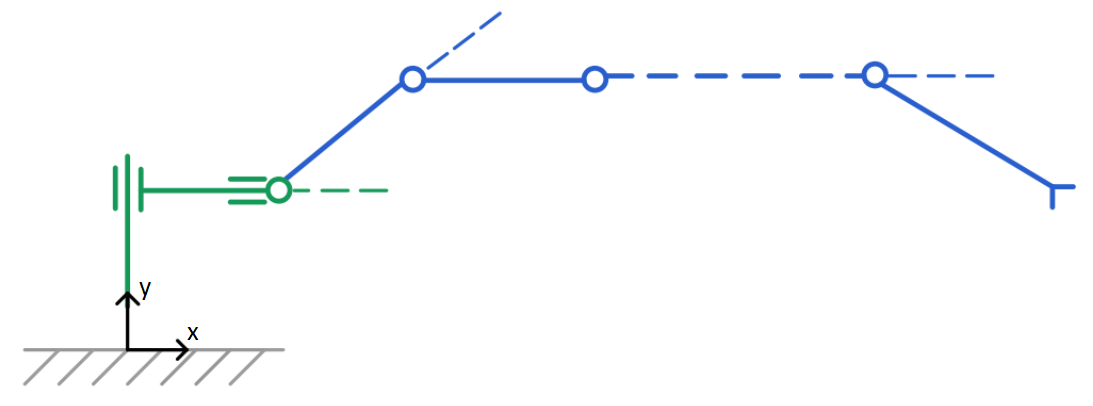
\includegraphics[width=0.9\textwidth]{figures/kinematics_noname.PNG}
    \caption{Model of snake robot with $n$ links}
    \label{fig:2_kin}
\end{figure}

%----------------------------------------------------------------------------------
%----------------------------------------------------------------------------------

\subsection{The environment}
The environment is the (x,y)-plane in Figure \ref{fig:2_kin}, and consists of nothing but the robot and the obstacles.

%----------------------------------------------------------------------------------
%----------------------------------------------------------------------------------


\subsection{The obstacles}

The obstacles are modeled as rigid points in the plane. However, as a consequence of the discrete nature of the simulator, there is a "safety barrier" around every obstacle defining the area in which contact is present. This contact is still modeled as a point contact. The barriers can be seen as the red circles in Figure \ref{fig:2_kin_obst}. The points the circles are surrounding are the actual obstacles.

\begin{figure}
    \centering
    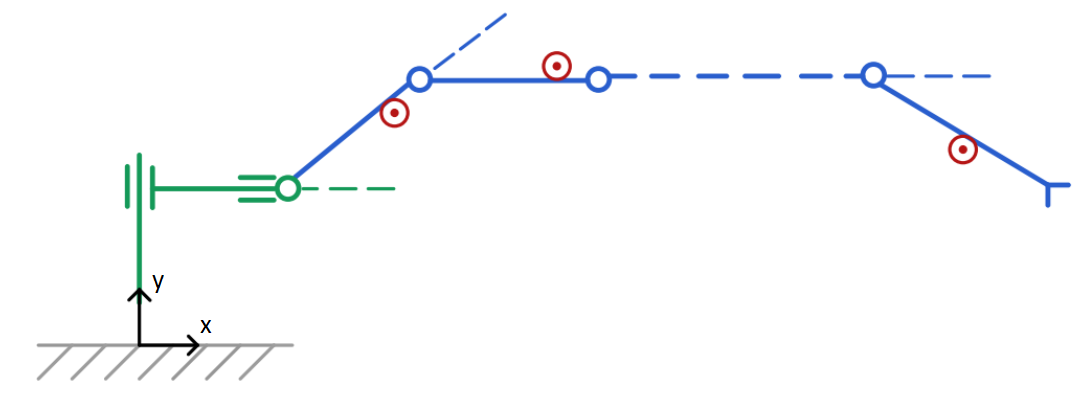
\includegraphics[width=0.9\textwidth]{figures/kinematics_obstacles_noname.PNG}
    \caption{Model of snake robot and obstacles}
    \label{fig:2_kin_obst}
\end{figure}

%----------------------------------------------------------------------------------
%----------------------------------------------------------------------------------

\subsection{The optimal path}

The path is in this report made out of straight lines and quadrants with radius equal to two times the link length $l$. There is no gap between these segments, following from the assumption of a continuous path.
\chapter{Background theory}\label{chapter:theory}

This chapter introduces relevant kinematics-, dynamics- and control theory for the snake robot specific case used in the development of the simulator. Further, the concepts of OAL and HPFC are explained to give insight into the motivation and structure of the simulator. Even though the idea of dynamical HPFC \cite{yoshikawa1987dynamic} is not applied in the project, it is presented as it is an essential part of the discussions in chapter \ref{ch:discussion}. Lastly, the methods for detecting contact with obstacles and adjusting to a predefined path are explained.


\section{Snake Robot Kinematics} \label{sec:kin}


The snake robot is modeled as a serial chain, which is a system of rigid bodies in which each member is connected to two others, except for the first and last members that are each connected to only one other member \cite{waldron2016kinematics}. As opposed to traditional robot manipulator models, the first joint in the the snake robot model is not physically connected to a base.


The vector of generalized coordinates $\mathbf{q}$ for a snake robot with $n$ links will be

\begin{equation} \label{eq:q}
    \mathbf{q} = 
    \begin{bmatrix}
        \phi_1 & \phi_2 & ... & \phi_n & x_0 & y_0
    \end{bmatrix}^T.
\end{equation}
\\
The coordinates $(x_0, y_0)$ and $\phi_1$ represent the position and orientation of the tail of the snake robot in reference to the base frame $(x,y)$. These coordinates cannot be directly controlled and will therefore be referred to as virtual coordinates. The generalized coordinates ${\phi_2, ... ,  \phi_n}$, corresponding to the actuated joints, refer to the angle of the following link relative to the preceding link. The number of generalized coordinates including two position coordinates and $n$ joint angles is $N = n+2$.

The model of the snake robot with the named variables are illustrated in figure \ref{fig:kin_name}. 
\begin{figure}
    \centering
    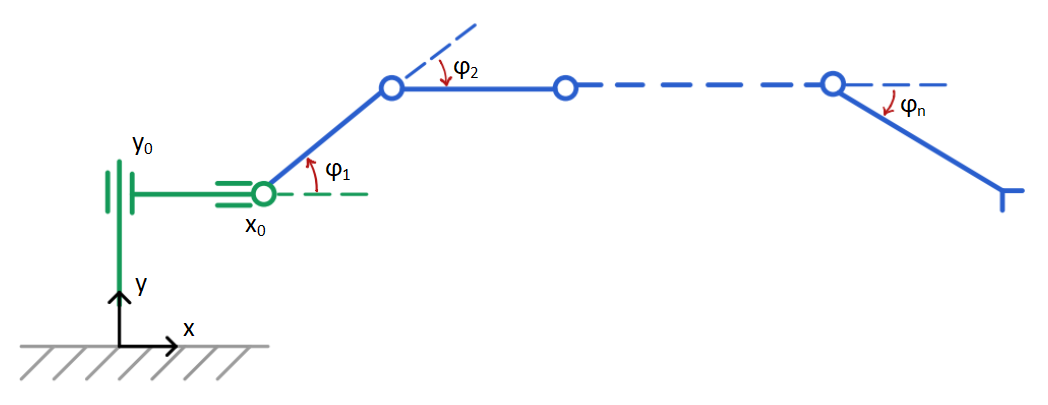
\includegraphics[width=0.9\textwidth]{figures/kinematics.PNG}
    \caption{Model of snake robot with notation}
    \label{fig:kin_name}
\end{figure}


Homogeneous transformation matrices are used to express the pose (position and orientation) of the links in relation to the base frame. This means that as long as the joint angles and size of the snake robot are known, the Cartesian positions can be calculated as well.
The homogeneous transformation matrix for the end point of link $i$ from the base frame $b$ is given by (\ref{eq:transformationmatrix}). The base frame will stay put regardless of motion of the robot. Note also that the link length $l$ is assumed equal for all the links.

\begin{equation} \label{eq:transformationmatrix}
    \textbf{T}_{b i} = \textbf{D}_x(x_0) \textbf{D}_y(y_0) \sum_{k=1}^{i} \textbf{R}_z(\phi_k) \textbf{D}_x(l)
\end{equation}
\\
The translation- and rotation matrices are given by

\begin{equation}\label{eq:trans_rot}
    \begin{split}
        \textbf{D}_x(x)& = 
        \begin{bmatrix}
            1 & 0 & x \\
            0 & 1 & 0 \\
            0 & 0 & 1
        \end{bmatrix}, \ \
        \textbf{D}_y(y) =
        \begin{bmatrix}
            1 & 0 & 0 \\
            0 & 1 & y \\
            0 & 0 & 1
        \end{bmatrix}, \ \
        \\&
        \\&\textbf{R}_z(\phi) =
        \begin{bmatrix}
            \cos{\phi} & -\sin{\phi} & 0 \\
            \sin{\phi} &  \cos{\phi} & 0 \\
            0          &  0          & 1
        \end{bmatrix}.
    \end{split}
\end{equation}
\\
The transformation matrix from the reference frame to the center of link $i$ can be found in the same manner. The only difference is that the very last translational matrix has to take the argument $l/2$ instead of $l$. This is useful to keep in mind as it will later be used for the derivation of the kinetic energy of the links.

As mentioned earlier, the transformation matrix $\textbf{T}_{b i}$ can be used to find the absolute orientation and position of the tip of link $i$ in the base frame.
The resulting matrix can be written on the form

\begin{equation}
    \textbf{T}_{b i} =
    \NORMAL{
    \begin{bmatrix}
        \textbf{R}_{b i}(\phi_{i,abs}) & \textbf{t}_{r i}^r \\
        \textbf{0}^T & 1
    \end{bmatrix} }.
\end{equation}
\\
The position is directly extracted from $\textbf{t}_{r i}^r = [x_i y_i]^T$. The orientation $\phi_{i,abs}$ is found by comparing $\textbf{R}_{b i}$ to $\textbf{R}_z$ and solving for $\phi_{i,abs}$.

Alternatively, one can directly compute the position of the center of a link $i$ from the expressions below

\begin{equation} \label{eq:pos}
    \begin{split}
        x_i &= x_0 + \sum_{k=1}^{i} l \cos{(\sum_{j=1}^{k} \phi_j)} \\
        y_i &= y_0 + \sum_{k=1}^{i} l \sin{(\sum_{j=1}^{k} \phi_j)},
    \end{split}
\end{equation}
\\
where $l$ is the link length and $i\leq n$.

\subsubsection{Forward and inverse instantaneous kinematics}\label{subseq:inst_fwd}

The well known Jacobian lets us transform between Cartesian and joint velocities. It is derived by taking the partial derivative of the $x$- and $y$ position of link $i\leq n$ with respect to all generalized coordinates

\begin{equation}\label{eq:Jc1}
    \mathbf{J_i} = 
    \HUGE{
    \begin{bmatrix}
        \frac{\partial x_i}{\partial q_1} & ... & \frac{\partial x_i}{\partial q_{N-1}} & \frac{\partial x_i}{\partial q_{N}} \\
        \frac{\partial y_i}{\partial q_1} & ... & \frac{\partial y_i}{\partial q_{N-1}} & \frac{\partial y_i}{\partial q_{N}} \\
    \end{bmatrix}
    }.
\end{equation}
\\
The relationship between the Cartesian velocity $\mathbf{v}$ of the point $(x_i, y_i)$ on the robot and the joint velocities $\mathbf{\dot{q}}$ can thus be written as 

\begin{equation}
    \mathbf{v_i = J_i(q) \dot{q}} \quad \textrm{ and } \quad \mathbf{\dot{q} = J_i(q)^\dagger v_i}.
\end{equation}
\\
The first equation is formally referred to as the forward instantaneous kinematics, whereas the second one is referred to as the inverse instantaneous kinematics.
$\mathbf{J(q)^\dagger}$ is the pseudo inverse of the Jacobian, which has to be used as a result of the Jacobian being non-square.

%------------------------------------------------------------------------------------------------

\subsection{Constrained kinematics}\label{seq:constr_kin}

%\hl{Virtual closed kinematic chain}\\
For the case in which the robot is in contact with the environment, the motion will be constrained. The obstacles found in the environment are modelled as single frictionless points. The only constraint imposed by the environment is that the robot cannot penetrate the obstacles. It can, however, both apply an arbitrary large force against them or move along them.

The model assumes that any link can be in contact with at most one obstacle at the time. To represent the mentioned constraint, we expand the vector of generalized coordinates with $n$ further elements, where $n$ is the number of links. The updated vector $\mathbf{q}$ is now

\begin{equation} \label{eq:q2}
    \mathbf{q} = 
    \begin{bmatrix}
        \phi_1 & \phi_2 & ... & \phi_n & x_0 & y_0 & d_{c,1} & d_{c,2} & ... & d_{c,n}
    \end{bmatrix}^T.
\end{equation}
\\
and $N = 2 + 2n$ is the new number of generalized coordinates.

The newly introduced coordinates $d_{c,1}, ... , d_{c,n} \geq 0$ represent the distance to the possible contact point from the corresponding joint. For instance, the coordinate $d_{c,2}$ is the distance between the second joint and the contact point measured along the second link, as illustrated in figure \ref{fig:3_obs_force}. Please note that every link might not be in contact with an obstacle, but the maximum number of coordinates is introduced in the interest of keeping the vector size constant. 
Seeing as there is no actuation force directly connected to the obstacle-related coordinates, they will be referred to as virtual joints or virtual coordinates.

The position of a contact point on link $i\leq n$ in the base frame can be derived through the corresponding transformation matrix (\ref{eq:obst_tfmatrix}).

\begin{equation} \label{eq:obst_tfmatrix}
    \textbf{T}_{b ci} = \textbf{D}_x(x_0) \textbf{D}_y(y_0) \sum_{k=1}^{i-1} (\textbf{R}_z(\phi_k) \textbf{D}_x(l)) \textbf{R}_z(\phi_i) \textbf{D}_x(d_{c,1})
\end{equation}
\\

\begin{figure}
    \centering
    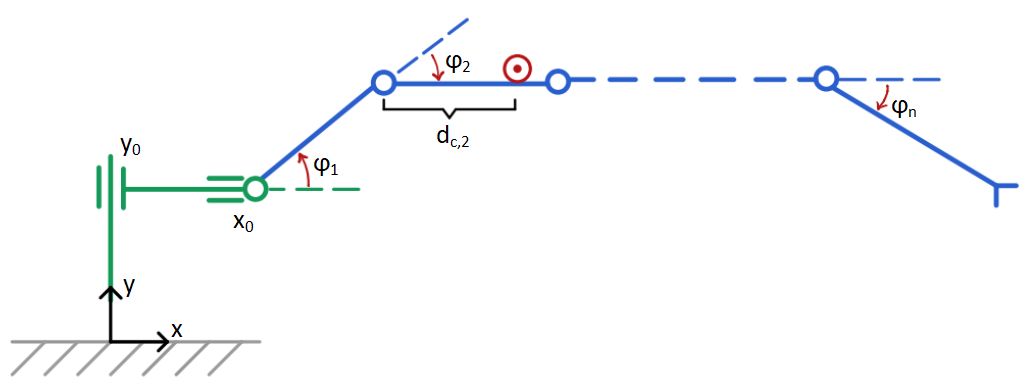
\includegraphics[width=0.9\textwidth]{figures/contact_point.PNG}
    \caption{Snake robot in contact with obstacle}
    \label{fig:3_obs_force}
\end{figure}


%------------------------------------------------------------------------------------------------

\subsubsection{Constrained instantaneous kinematics}\label{subseq:constr_inst}

The Jacobian matrix related to the velocity of the contact point can be derived in the same manner as in the unconstrained case. The only difference is that the partial differentiation of the contact point $(x_c,y_c)$ now is taken with respect to the extended vector of generalized coordinates (\ref{eq:q2}). The result for a contact point on link $i$ is thus

\begin{equation}\label{eq:Jac_constr}
    J_{c,i} = 
    \HUGE{
    \begin{bmatrix}
        \frac{\partial x_{c,i}}{\partial \phi_2} & ... & \frac{\partial x_{c,i}}{\partial q_{N-1}} & \frac{\partial x_{c,i}}{\partial q_N} \\
        \frac{\partial y_{c,i}}{\partial \phi_2} & ... & \frac{\partial y_{c,i}}{\partial q_{N-1}} & \frac{\partial y_{c,i}}{\partial q_N} \\
    \end{bmatrix}
    }.
\end{equation}
\\
This Jacobian will end up being quite sparse, seeing as the coordinate of a contact point is independent of all other contact coordinates. This is a property that can be exploited using sparse solvers if the snake robot has a large amount of links.

The relationships between the Cartesian velocity of a contact point on link $i \leq n$ and the joint velocities can now be expressed as

\begin{equation}
    \mathbf{v_{c,i} = J_{c,i}(q) \dot{q}} \quad \textrm{ and } \quad \mathbf{\dot{q} = J_{c,i}(q)^\dagger v_{c,i}}.
\end{equation}


%------------------------------------------------------------------------------------------------
%------------------------------------------------------------------------------------------------

\section{Snake Robot Dynamics} \label{sec:dyn}

The snake robot has $n-1$ actuators that all can apply torques to their corresponding joints. The dynamics describe how the robot moves in response to these actuator forces. For simplicity, it is assumed that the actuators do not have dynamics of their own and, hence, arbitrary torques can be commanded at the joints of the robot \cite{murray2017mathematical}.

The dynamics of the snake robot will be expressed using the joint space equations of motion formulation:

\begin{equation}
    \mathbf{M(q)\ddot{q} + C(q, \dot{q}) + g(q)} = \boldsymbol{\tau}.
\end{equation}
\\
Because the movement is restricted to the 2D plane, the gravitational term $\mathbf{g(q)}$ can be neglected and we can rewrite the equations of motion to

\begin{equation}\label{eq:eom}
    \mathbf{M(q)\ddot{q} + C(q, \dot{q})} = \boldsymbol{\tau},
\end{equation}
\\
where $\mathbf{M(q)}$ and $\mathbf{C(q,\dot{q})}$ is the mass matrix and Coriolis matrix respectively.
$\boldsymbol{\tau}$ is the vector of generalized torques corresponding to the generalized coordinates (\ref{eq:q}). Please note that the elements corresponding to the virtual coordinates will be zero at all times.

Solving (\ref{eq:eom}) with respect to $\mathbf{\ddot{q}}$ yields

\begin{equation}\label{eq:eom_qdd}
    \mathbf{\ddot{q}} = \mathbf{M^{-1}(q)}( \boldsymbol{\tau} - \mathbf{C(q, \dot{q})}).
\end{equation}
\\
There exists several methods for finding the equations of motion for a robot.The Euler-Lagrange method \cite{lynch2017modern} is chosen here, which is based on the difference in kinetic energy ($K$) and potential energy ($P$) of the system, also known as the Lagrangian:

\begin{equation}
    L = K - P.
\end{equation}
\\
The equations of motion can now be expressed as a second order partial differential equation:

\begin{equation} \label{eq:Lagrange}
    \frac{d}{d t} \frac{\partial L}{\partial \mathbf{\dot{q}}} - \frac{\partial L}{\partial \mathbf{q}} = \boldsymbol{\tau}.
\end{equation}
\\
Again, we can make simplifications from the restricted movement in the world and neglect the potential energy $P$. The Lagrangian is therefore simply equal to the kinetic energy, which is the sum of the kinetic energy for every link \cite{rezapour2014path}. Furthermore, the kinetic energy for one link $i$ is divided into two parts, $K_{translational}$ and $K_{rotational}$.
We can now express the kinetic energy as

\begin{equation}
    K = \sum_{i=1}^{n} (K_{translational,i} + K_{rotational,i}),
\end{equation}
\\
where the translational and rotational kinetic energy is given in (\ref{eq:k_trans}) and (\ref{eq:k_rot}) respectively.

\begin{equation} \label{eq:k_trans}
    K_{translational,i} = \frac{1}{2} m (\dot{x}_i^2 + \dot{y}_i^2)
\end{equation}
\\
Here $m$ is the link mass, and $(\dot{x}_i, \dot{y}_i)$ make out the velocity of the center of the link found by differentiating (\ref{eq:pos}) with respect to time. 

\begin{equation} \label{eq:k_rot}
    K_{rotational,i} = \frac{1}{2}I\dot{\phi_i}^2
\end{equation}
\\
$\dot{\phi}_i$ is the joint velocity of link $i$. Furthermore, every link has the same moment of inertia, namely $I = m (1/12)ml^2$. This is the moment of inertia of a rod, corresponding to the moment of inertia of a cylinder with zero radius \cite{lynch2017modern}.


%------------------------------------------------------------------------------------------------

\subsection{Constrained dynamics}\label{subseq:constr_dyn}

The generalized torques from the right side of (\ref{eq:eom}) can be split into two parts whenever there is contact between the robot and the environment, namely a component resulting from the control inputs (motor torques), $\boldsymbol{\tau_{m}}$, and a component resulting from the external forces acting on the robot, $\boldsymbol{\tau_{c}}$ \cite{rezapour2014path}. The generalized torques can thus be written as

\begin{equation}
    \boldsymbol{\tau} = \boldsymbol{\tau_{m}} + \boldsymbol{\tau_{c}}.
\end{equation}
\\
According to Holden \cite{holden2014optimal}, the force from an obstacle acting on a link is two-fold: one normal to the link and one tangent to the link. The force tangent to the link is due to friction and will therefore be neglected in this project. The remaining normal force is preventing the link from moving into the obstacle when the robot itself is applying a force to the obstacle. The external force in the frame of link $i$ acting on link $i$ is denoted $\mathbf{f}^i_{c,i}$ and can be written as

\begin{equation}
    \mathbf{f}^i_{c,i}=
    \begin{bmatrix}
        0 \\
        f^i_{c,i,y}
    \end{bmatrix}.
\end{equation}
\\
The following derivations are inspired by \cite{rezapour2014path}. The force $\mathbf{f}^i_c$ can be expressed in the base frame by using the rotation matrix from (\ref{eq:trans_rot}):

\begin{equation}
    \mathbf{f}^b_{c,i} = \mathbf{R}_z(\alpha_i) \mathbf{f}^i_{c,i},
\end{equation}
\\
where $\alpha_i$ is the angle of link $i$ related to the base frame $b$. It can be found by $\alpha_i = \sum_{k=1}^{i} \phi_k$.

The contact Jacobian (\ref{eq:Jac_constr}) can be used to find the generalized external torque as a result of the external forces:

\begin{equation}
    \boldsymbol{\tau_c} = \sum_{i=1}^{n} \mathbf{J}^T_{c,i} \mathbf{f}^b_{c,i}.
\end{equation}



%------------------------------------------------------------------------------------------------
%------------------------------------------------------------------------------------------------

%\section{Obstacle contact force}



%The force the obstacle is pushing back with on link $m$ is simply denoted , where $\mathbf{\norm{f_m} = \norm{f_{c,m}}}$. The sign of the force will also depend on which side of the link the obstacle is lying on \cite{holden2014optimal}. The sign is here denoted by $\gamma_m$, where $\gamma_m > 0$ for obstacles to the right of the link and vice versa. The force acting on link $m$ is thus

%The different forces acting on the robot can be stacked in the matrix $\mathbf{F_m}$ and the corresponding transposed Jacobians can be stacked in the matrix $\mathbf{J_c}$. When all the forces from the different obstacles are found, the corresponding torques can be added to the equations of motion to obtain the resulting behavior of the robot. The updated equations of motion are

%The joint torque $\boldsymbol{\tau}$ from the robot is now acting on both the joints of the robot and on the obstacle. From basic physics theory we know that for rigid bodies, the force between two bodies are equal opposites. This means that the robot joint torque $\boldsymbol{\tau}$ has a component which will be cancelled by the obstacle force/torque. We call this component $\boldsymbol{\tau}_c$. The remaining torque $\boldsymbol{\tau_a}$ will contribute to accelerating the links of the robot. Hence, we can express the joint torque on the format


%------------------------------------------------------------------------------------------------
%------------------------------------------------------------------------------------------------

\section{Computed torque control}
The content of this section is taken from chapter 11 of Modern Robotics \cite{lynch2017modernCompTorque}.

\subsection{PD control}
A common feedback controller is linear proportional-derivative control, or PD-control:

\begin{equation}\label{eq:pd}
    \boldsymbol{\tau} = \mathbf{K_p q_e + K_d \dot{q}_e}.
\end{equation}
\\
The control gains $\mathbf{K_p}$ and $\mathbf{K_d}$ are positive diagonal matrices. The proportional gain $\mathbf{K_p}$ acts as a virtual spring that tries to reduce the position error $\mathbf{q_e = q_d - q}$, where $\mathbf{q_d}$ is the desired joint angles. The derivative gain $\mathbf{K_d}$ acts as a virtual damper that tries to reduce the velocity error $\mathbf{\dot{q}_e = \dot{q}_d - \dot{q}}$.

Substituting the PD control law into the dynamics (\ref{eq:eom}) yields

\begin{equation}\label{eq:control1}
    \mathbf{M \ddot{q} + C(q, \dot{q}) = K_p (q_d - q) + K_d (\dot{q}_d - \dot{q})}.
\end{equation}
\\
The damping ratio $\zeta$ and natural frequency $\omega_n$ of this system is given as:

\begin{equation}\label{eq:control2}
    \zeta = \mathbf{\frac{K_d}{2 \sqrt{K_p M(q)}}} \quad  \
    \textrm{and} \quad \
    \omega_n = \mathbf{\sqrt{\frac{K_p}{M(q)}}}.
\end{equation}
\\
We know that $\zeta = 1$ to satisfy critical damping. Furthermore, $\mathbf{K_p}$ should be chosen as high as possible for a fast response.

\subsection{Feedforward control}
%(Modern Robotics 11.4.1.2)\\
Another strategy for trajectory following is to use the model of the robot's dynamics (\ref{eq:eom}) to proactively generate torques instead of waiting for errors. The feedforward torque is calculated as 

\begin{equation}\label{eq:feedforward}
    \boldsymbol{\tau} = \mathbf{\Tilde{M}(q_d)\ddot{q}_d + \Tilde{C}(q_d, \dot{q}_d)},
\end{equation}
\\
where the model is perfect if $\mathbf{\Tilde{M}(q) = M(q)}$ and $\mathbf{\Tilde{C}(q,\dot{q}) = C(q,\dot{q})}$.


\subsection{Feedforward and feedback linearization} \label{subsec:comp_torque}
%(Modern Robotics 11.4.1.3) \\

As no model of the robot and environment will be perfect, it is not sufficient to use pure feedforward control. Combining the PD controller (\ref{eq:pd}), with a proper choice of PD gains, and a feedforward term (\ref{eq:feedforward}) will ensure exponential decay of the trajectory error (not just setpoint error).

Since $\mathbf{\ddot{q}_e = \ddot{q}_d - \ddot{q}}$, we get

\begin{equation}\label{eq:qdd}
    \mathbf{\ddot{q} = \ddot{q}_d + K_d \dot{q}_e + K_p q_e}.
\end{equation}
\\
From substituting (\ref{eq:qdd}) into the robot dynamics (\ref{eq:eom}) we get the computed torque controller, also known as feedforward plus feedback linearizing controller:

\begin{equation}\label{eq:controllaw}
    \boldsymbol{\tau} = \mathbf{\Tilde{M}(q) (\ddot{q}_d + K_d \dot{q}_e + K_p q_e) + \Tilde{C}(q,\dot{q})}.
\end{equation}
\\
A block diagram of the resulting control (\ref{eq:controllaw}) is shown in figure \ref{fig:block-diag-torque}.

\begin{figure}
    \centering
    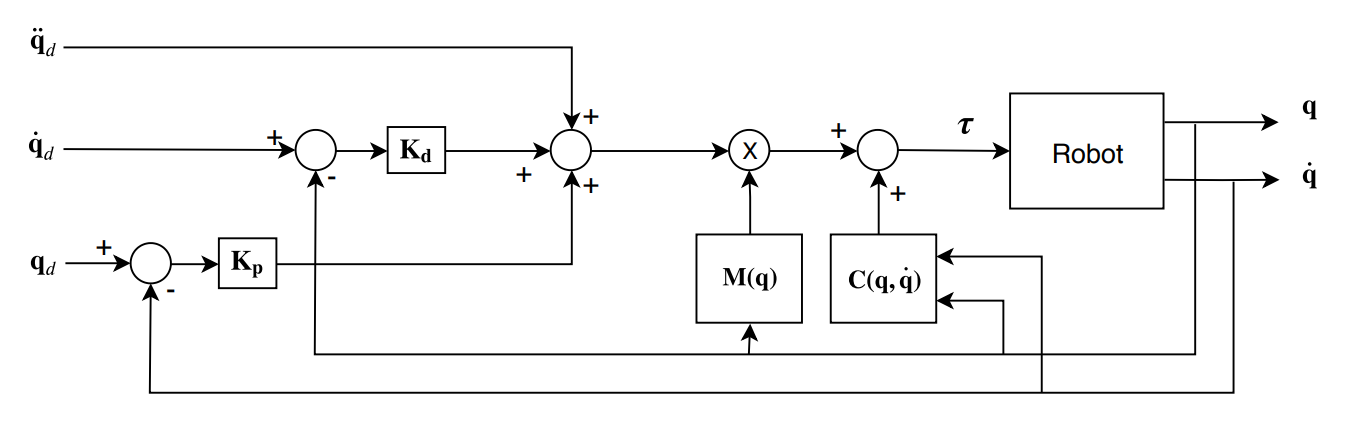
\includegraphics[width=0.9\textwidth]{figures/comptorque.PNG}
    \caption{Computed torque control block diagram}
    \label{fig:block-diag-torque}
\end{figure}

%-----------------------------------------------------------------------------------
%-----------------------------------------------------------------------------------
%-----------------------------------------------------------------------------------




\section{Obstacle-Aided Locomotion (OAL)}

Instead of avoiding physical contact between the robot and obstacles, obstacle aided locomotion aims at profiting from it by using the obstacles as push-points to propel itself forward. OAL was first introduced by Transeth et al. in 2008 \cite{transeth2008snake}. The motivation behind this method was based in the ability of biological snakes to utilize irregularities in the terrain for more efficient locomotion.

Liljebäck et al. \cite{liljeback2012snake} describe two major challenges related to OAL:
\begin{enumerate}
  \item It is unknown in advance when and where the snake robot will make contact with its environment.
  \item The development of a strategy for adjusting the shape of the robot so that forward propulsion is achieved in any given contact situation.
\end{enumerate}
Furthermore, \cite{liljeback2012snake} state the following hypothesis:
\begin{quote}
   \textit{ Obstacle-aided snake robot locomotion can be achieved by producing body shape changes where the links in contact with obstacles are rotated so that the components of the contact forces in the desired direction of motion are increased.}
\end{quote}

Holden et al. \cite{holden2014optimal} address the second challenge by formulating an optimization problem that seeks to minimize energy consumption while achieving propulsion along a user-defined desired path. The output of this optimization is the optimal motor torque inputs. In addition to a user-defined path, this method assumes that the desired link angles at the obstacles are given.

Bayraktaroglu \cite{bayraktaroglu2004understanding} mentions that only the trajectory of the leading link should be arbitrarily determined. Moreover, \cite{bayraktaroglu2004understanding} states that in a steady smooth motion, it must be computed as a function of available push-points for the next contact. The desired position and orientation of the following links are those that mimic the motion of the leading link.




%------------------------------------------------------------------------------------------------
%------------------------------------------------------------------------------------------------


\section{Hybrid Position/Force Control (HPFC)}

The goal of the snake robot is to push against obstacles in a fashion that yields forward propulsion along a path. Consequently, the robot will have to curve itself along the path whilst applying a force to the obstacles considered advantageous. The behavior of the robot has to comprise with the constraints arising from the contact, which further motivates the use of hybrid position/force control (HPFC).
%Pure motion control for controlling this kind of interaction is prone to failure as it would require a perfect model of both the robot and the environment.
%In practice, the planning errors for controlling this kind of interaction may give rise to a contact force and moment causing a deviation of the desired trajectory. The control system will try to reduce this error and increase the force until it reaches the saturation and the robot possibly brakes. (Chapter 7, Springer Handbook of Robotics)
%\hl{But we have a perfect model for the simulation!}

HPFC is not a control method per se, but rather a method for determining when and in which directions force- or motion control should be applied. We wish to control motion along the unconstrained motion directions and force along the constrained motion directions. There exists different approached to this problem. One is the use of selection matrices, introduced by Raibert and Craig \cite{raibert1981hybrid}. The disadvantage of this approach is that the directions in which force and motion should be controlled has to be recalculated for every step, and is no simple procedure. A second approach was introduced by West and Asada \cite{west1985method}, in which two projection matrices are used as filters in joint space to automatically select between position- and force controlled vectors. The rest of the section covers this method and is based on the paper of West and Asada.

\subsection{Constrained  motion}\label{subseq:HPFC}
Like mentioned above, velocity and force can be controlled in the directions in which they are not constrained. The end effector space is divided into two orthogonal domains, a position domain and a force domain, which are complementary to the directions of the corresponding constraints at the end effector. If there is contact with the environment, motion cannot be controlled freely. If there, on the other hand, is no contact, there is no direction in which the robot can apply a force and the robot is force constrained. Ergo, the force and motion control directions do not overlap and the domains are orthogonal. This means that position and force can be controlled independently and arbitrarily in these domains.

The following relationships are known from sections \ref{seq:constr_kin} and \ref{subseq:constr_dyn}. 

\begin{equation}
	\mathbf{v = J \dot{q}} \textrm{,} \quad  \  \boldsymbol{\tau} \mathbf{= J^T f}
\end{equation}
\\
An important observation is that constraints due to contact with the environment are constraints due to a closed kinematic chain. In the snake robot case there might not always be two points in contact with the environment. It is however possible to define a virtual closed kinematic chain where the robot is connected to the base with the virtual joint variables $x_0$, $y_0$ and $\phi_1$.
A separate Jacobian has been calculated for each closed kinematic chain, as explained in \ref{subseq:constr_inst}.
%These Jacobians are denoted $\mathbf{J_{ci}}$, where $i = 1, .., k$ is the number of independent closed kinematic chains.
Since the motion is constrained at a contact point we have the relationships

\begin{equation} \label{eq:constr_dyns}
    \mathbf{\dot{v}_{ci} = J_{ci} \dot{q} = 0}.
\end{equation}
\\
The solution to (\ref{eq:constr_dyns}) can be proven to be

\begin{equation}
    \mathbf{\dot{q} = (I - J_{ci}^+ J_{ci}) y},
\end{equation}
\\
where $\mathbf{y}$ can be an arbitrary vector, as it will yield zero end effector motion. Furthermore, since the matrix $\mathbf{J_{ci}}$ might be non square, the pseudo inverse $\mathbf{J_{ci}^+}$ is used.
For a closed kinematic chain, the work done at the end of the chain must also be zero. Therefore, the sum of the work done by each of the joints must be zero:

\begin{equation} \label{eq:zero_joint_work}
    \boldsymbol{\tau^T} \mathbf{\dot{q}} = \boldsymbol{\tau^T} \mathbf{(I - J_{ci}^+ J_{ci}) y = 0}.
\end{equation}
\\
(\ref{eq:zero_joint_work}) has the general solution

\begin{equation}
   \boldsymbol{\tau}  \mathbf{= (J_{ci}^+ J_{ci})^T z},
\end{equation}
\\
where $\mathbf{z}$ can be an arbitrary vector.

The allowable motion is now characterized by $\mathbf{[I - J_{ci}^+ J_{ci}]}$ and the allowable forces by $\mathbf{[J_{ci}^+ J_{ci}]^T}$. These matrices are orthogonal projectors in joint space onto the allowable position and force variations respectively. For a further explanation of this result, please see chapter 5 of \cite{west1985method}. The projectors will be abbreviated to

\begin{equation}\label{eq:proj_mtrices}
    \mathbf{
    \prescript{j}{ap}{P} = [I - J_{ci}^+ J_{ci}] \ \ \quad \textrm{and} \quad
    \prescript{j}{af}{P} = [J_{ci}^+ J_{ci}]^T = [I - (\prescript{j}{ap}{P})^T]
    }.
\end{equation}
\\
The superscript $j$ denotes joint space, and $ap$ and $af$ stand for allowable positions and allowable forces respectively.

\subsection{Multiple constraints}\label{subseq:mult_contacts}

If there are several contact points, projection matrices are calculated for each constraint, and the final projection matrices are found by taking the union and intersect of the different $\prescript{j}{af}{P}$ and $\prescript{j}{ap}{P}$ respectively.

\subsection{Passive joints}
The constraints (obstacles) are modeled as virtual joints, described in \ref{seq:constr_kin}. These joints are always passive, and since the corresponding forces are uncontrollable, they are always zero. To satisfy the additional constraint imposed by the passive joints, one can use a diagonal matrix $\mathbf{A}$ with ones on the diagonal indicating active joints. Another approach is to control the contact force at the contact point to satisfy the requirement that the force in the passive joints is zero.

\subsection{Dynamic HPFC}\label{subseq:dynhpfc}

This section briefly explains the dynamic hybrid control method based on the paper of Yoshikawa \cite{yoshikawa1987dynamic}. 

For describing the dynamics of the constraint manipulator, the constraints at the end effector are described by a set of constraint hypersurfaces before the equations of motion are derived. A given end effector constraint is expressed by a set of $m$ hypersurfaces:

\begin{equation}\label{eq:dynhpfc0}
    p_i(\mathbf{r}) = 0, \quad i = 1, 2, ..., m,
\end{equation}
\\
where $\mathbf{r}$ is the end effector position in a fixed frame. Furthermore, the relation between the joint variables $\mathbf{q}$ and the end effector position $r$ is given by

\begin{equation}\label{eq:dynhpfc1}
    \mathbf{r = c(q)}.
\end{equation}
\\
Differentiating $\mathbf{c(q)}$ with respect to $\mathbf{q}$ gives the familiar Jacobian matrix $\mathbf{J}$.
Differentiating (\ref{eq:dynhpfc1}) with respect to time gives

\begin{equation}\label{eq:dynhpfc2}
    \mathbf{E_F \dot{r}} = 0,
\end{equation}
\\
where $\mathbf{E_F}$ consists of the unit normal vectors to the hypersurfaces (\ref{eq:dynhpfc0}).

The force exerted on the constraint surface by the end effector in the base frame $b$ is denoted $\mathbf{f}^b \in \mathbb{R}^6$. Since the method assumes no friction between the surface and effector, then from the principle of virtual work $\mathbf{f}^b$ satisfies

\begin{equation}\label{eq:dynhpfc3}
    \mathbf{v}^T \mathbf{f}^b = 0,
\end{equation}
\\
where $\mathbf{v}$ is the end effector velocity $\mathbf{T\dot{r}}$. (\ref{eq:dynhpfc2}) can thus be written

\begin{equation}\label{eq:dynhpfc4}
    \mathbf{E_F T^{-1} v} = 0.    
\end{equation}
\\
Eventually, the force $\mathbf{f}^b$, given (\ref{eq:dynhpfc3}) and (\ref{eq:dynhpfc4}), can be written 

\begin{equation}
    \mathbf{f}^b = \mathbf{E_F T^{-1}} \mathbf{f}_F,
\end{equation}
\\
where $\mathbf{f}_F \in \mathbb{R}^m$ is an unknown vector. It can be shown that the vector $\mathbf{-f}_F$ takes the same value as the Lagrange multiplier $\boldsymbol{\lambda}$ of the the Lagrange equations of motion for the manipulator under the following constraint:

\begin{equation}
    \Tilde{p}_i(\mathbf{c(q)}) = 0, \quad i = 1, 2, ..., m,
\end{equation}
\\
where $\Tilde{p}_i(\mathbf{r}) = p_i(\mathbf{r})/||dp_i(\mathbf{r})/d\mathbf{r}||$.

The dynamics can now be expressed as

\begin{equation}
    \mathbf{M(q)\ddot{q} + C(q,\dot{q}) + g(q)} = \boldsymbol{\tau_m} + \mathbf{J^T}(d\Tilde{\mathbf{p}}/d\mathbf{r})^T \boldsymbol{\lambda},
\end{equation}
\\
where $\boldsymbol{\tau_m}$ is the joint driving force. The left hand side of the equation is the general manipulator dynamics.


%---------------------------------------------------------------------------------------------
%---------------------------------------------------------------------------------------------

\subsection{HPFC for Snake Robots}\label{subseq:snakeHPFC}

%(OE's notat) "HPFC arose from a situation where robots exhibited increasing sensor capabilities, especially with respect to contact force measurements, capitalising on this technological progress to improve and simplify the control task from both a theoretical and practical perspective. Today we see a similar situation in snake robotics, in that a snake robot can be equipped with sensors that enable perception of the robot's configuration and position in space, the geometry and mechanical properties of its immediate environment (6, F. Sanfilippo), and contact forces arising between the robot and the surroundings (7. P. Liljebäck). The present project aims at capitalizing on this progress to establish compliant, robust, physics based snake robot locomotion algorithms that can be put to practical use in terrestrial snake robot applications."

The joint torques of the robot have to be calculated in a way that allows the robot to apply forces in certain directions while simultaneously positioning itself along the path. In order to find these torques, it is necessary to know in which direction the mentioned actions are allowable.

A snake robot lying alongside an obstacle is able to move along the obstacle. It is however unable to move through the obstacle. Hence, the direction in which the obstacle lies, limits the allowable position space. On the contrary, the allowable force space is restricted to the same direction. 
This is also sensible, as it makes no sense to attempt to apply a force in the direction of free space. Such and attempt would solely yield an uncontrolled acceleration of the robot joints.




The directions in which the robot can apply forces to obstacles is referred to as the allowable force space $\mathbb{F}$, and the directions in which it can move freely is referred to as the allowable position or motion space $\mathbb{M}$. The idea of Raibert and Craig \cite{raibert1981hybrid} was that these spaces both make out the subspaces of a bigger task space $\mathbb{T}$, which in the snake robot case is propulsion along a predefined path. The two subspaces are orthogonal, i.e. $\mathbb{T}=\mathbb{F}\cup\mathbb{M}$, $\mathbb{F}\perp\mathbb{M}$.

Stavdahl \cite{StavdahlNote} introduces a ternary decomposition of the task space based on the fact that not all force interaction between the robot and the obstacles will yield propulsion. In some robot configurations, the reaction forces from the obstacles might even lead to a lock and increasing forces between the rigid bodies that might eventually lead to the robot breaking. The reaction forces illustrated in figure \ref{fig:noprop} have no component that would push the robot in the forward direction. The robot could however bend its links and thus change its shape. Consequently it would be able to apply a torque yielding propulsion.

\begin{figure}[h!]
    \centering
    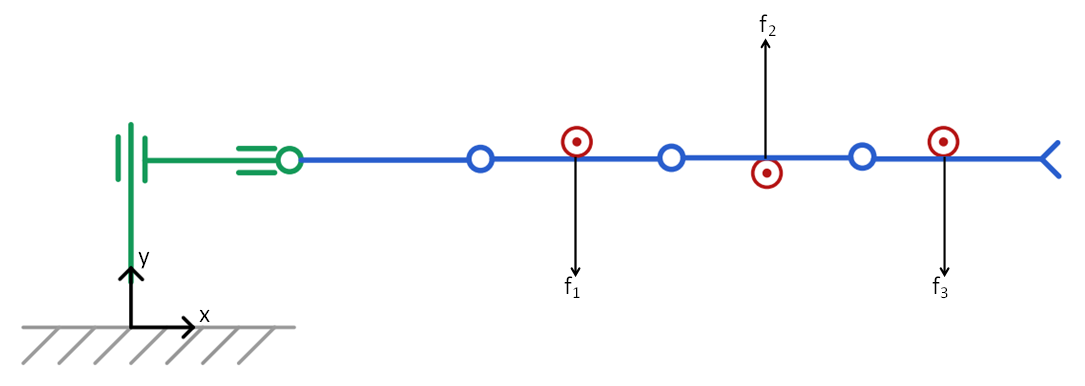
\includegraphics[width=0.8\textwidth]{figures/no_propulsion.PNG}
    \caption{Configuration of the snake robot and obstacles yielding no propulsion}
    \label{fig:noprop}
\end{figure}

In other words there is a subspace of the force space which will not contribute to propulsion. \cite{StavdahlNote} denotes this as the \textbf{constraint space} $\mathbb{C}$. The subspace within which we achieve forward motion of the head is denoted the \textbf{propulsion space} $\mathbb{P}$. The remaining subspace, the \textbf{shape space} $\mathbb{S}$, is the space in which the joint torques simply change the shape configuration of the robot.

Finally, knowledge about the specified spaces may be exploited in planning of a path from one point to another. In particular, it can be used to design an optimal path that maximizes the propulsion space. When the corresponding optimal forces are known, HPFC can be used to realise these forces while adjusting the shape of the robot to the path.

%---------------------------------------------------------------------------------------
%---------------------------------------------------------------------------------------
%---------------------------------------------------------------------------------------

\section{Projection onto path}\label{sec:pathproj}
In order for the robot to adjust its shape to fit the desired path, its controller is dependent on knowing the joint angles that fulfill this task. The desired joint angles are found by projecting the snake onto the predefined path. It is assumed that the 2D path is known at all times. Since the path has no width it is possible to simply find the shortest distance from a joint to the path to determine where the joint \textit{should have} been. This distance is called $BC$ and is illustrated in figure \ref{fig:path_proj}. The path can be discretized to consist of points along the lines and curves defining the path.

\begin{figure}[h!]
    \centering
    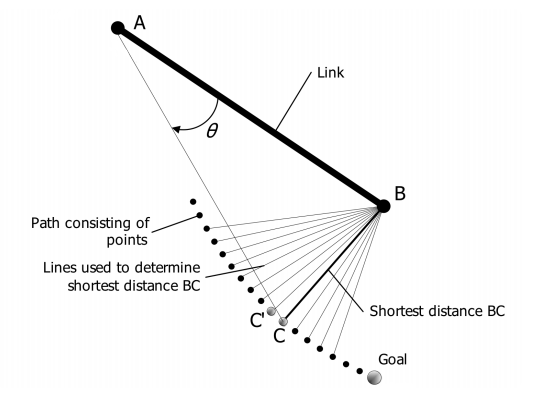
\includegraphics[width=0.7\textwidth]{figures/path_proj.PNG}
    \caption{Shortest distance from joint to path \cite{conkur2008path}}
    \label{fig:path_proj}
\end{figure}

The shortest distance is chosen by numerically comparing all the line segments from the joint to a piece of the path seen as relevant based on the position of the robot. When this point is known, the angle $\theta$ can be determined by trigonometrical properties. We know that the distance $AB$ will equal the length of a link $l$. The points $A$ and $B$ are respectively the positions of the preceding joint and joint to be projected. The distance $AC$ is now called $a$ and the distance $BC$ is called $b$. From the law of cosine we have that

\begin{equation}
    \cos{(\theta)} = \frac{l^2 + a^2 - b^2}{2lb}.
\end{equation}
\\
Note that this expression will be invalid if the shortest distance from the joint to the path is zero, meaning the joint is already on the path. There is however no need to perform a projection if there is no deviation from the path. In the case of very precise calculation, the joint and the path will never overlap completely. One can however introduce a very small width around the path in which the joint is considered to be on the path. This is equivalent to the threshold introduced in \cite{conkur2008path}, where an angle deviation $\theta$ lower than the threshold is ignored.

%The angle $\theta$ is the deviation from the path an thus the joint angle error.
Because we assume no explicit information about which side (left/right) of the path the joints are lying on, we are unfamiliar with the sign of $\theta$. The easiest way to solve this in a computer program is simply comparing the result of rotation around $A$ with both the positive and negative angle option. The link $AB$ is rotated using the rotation matrix $\mathbf{R_z}$, defined in (\ref{eq:trans_rot}). The resulting projected points are thus

\begin{equation}
    C^+ = A + \mathbf{R_z}(\theta)AB \quad \text{and} \quad
    C^- = A + \mathbf{R_z}(-\theta)AB.
\end{equation}
\\
The angle with the corresponding point closest to $C$ is chosen.


%-----------------------------------------------------------------------------------
%-----------------------------------------------------------------------------------
%-----------------------------------------------------------------------------------

\section{Contact detection}

Before the consequence of an interaction is calculated, the point of contact (if any) has to be determined. This is done by projecting the obstacle point onto the closest link. The distance from the obstacle to the projected point is then compared to the safety radius $r_{safety}$ around each obstacle. This safety radius is to avoid the scenario in which the robot in a discrete time step moves to the opposite side of the obstacle point. Consequently, we get the relation in \ref{eq:obstrad}. The parameters are shown in figure \ref{fig:obstrad}.This figure shows a case in which contact is established.

\begin{equation}\label{eq:obstrad}
    contact =
    \begin{cases}
        1 & \text{if $pc \leq r_{safety}$}\\
        0 & \text{else}
    \end{cases}
\end{equation}
\\
\begin{figure}
    \centering
    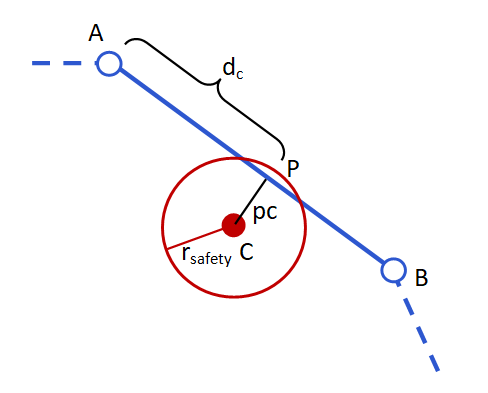
\includegraphics[width=0.6\textwidth]{figures/obst_radius.PNG}
    \caption{Robot link and obstacle with safety radius}
    \label{fig:obstrad}
\end{figure}
If link $i$ is considered in contact with an obstacle, the distance $d_{c,i}$, which is a generalized coordinate introduced in \ref{seq:constr_kin}, equals $|AP|$ (see figure \ref{fig:obstrad}).


\chapter{The simulator}\label{ch:simulator}

The purpose of the simulator is to visualize the movement of a simple snake robot model progressing according to a predefined path and obstacles in the environment. Because the tested concepts are rather experimental and go in the direction of a proof-of-concept, the whole simulator is developed from scratch in MATLAB. The process of coding the simulator has also been a great resource for studying these concepts and the general theory of snake robots. The following limitations coming from this approach are presented below.
This chapter also aims at describing how the simulator is structured and can be used, as well as explaining particular code snippets in more detail. Moreover, it provides an overview of how the mathematical background is applied.

%-----------------------------------------------------------------------------------
%-----------------------------------------------------------------------------------

\section{Simplifications and limitations}

Expressing the complete dynamics of the system includes explicitly finding the part of the joint torques that are not directly applied to the robot joints, but rather a force acting on the external obstacles. In other words, the torque would have to be separated in a component belonging to the constraint- or propulsion space and a component that belongs to the shape space (see \ref{subseq:snakeHPFC}).

This challenge, combined with a strict time schedule, has led to a simplification in the development of the simulator. In the simulator, the movement of the robot is first calculated under the assumption that no obstacle is present. To account for this, the interaction forces are implicitly considered through mapping to the allowable position space. This means that if the robot is in contact with the environment, the joint velocities are influenced accordingly and thus also the joint angles. The consequences of the simplification are discussed in chapter \ref{ch:discussion}.

Like in any computer simulation, the time is discretized. This leads to inaccuracies, especially for fast motions. To minimize the effect of the simplification, the sampling time may be decreased. 

Furthermore, the projection onto the desired path assumes that the robot is sufficiently close to the path to get back to it. The calculated desired angles for joints very far away from the path might therefore not lead to advantageous behaviour. The projection also assumes that the links of the robot are chronologically aligned along the path. This means that if the robot is for instance curled up, the projection will fail to align the robot.


%-----------------------------------------------------------------------------------
%-----------------------------------------------------------------------------------

\section{Program flow}

The program flow is illustrated in the diagram figure \ref{fig:prog_flow}. The blue rectangles represent functions, and the data connected to the outgoing arrows are computed output variables. From the diagram, it is noticeable that the program runs in a loop after initialization, constantly controlling the robot towards the path while adapting to its environment (the obstacles).

Initialization is performed based on the given snake robot and obstacle configurations. Furthermore, the joint acceleration $\mathbf{\ddot{q}}$ of the robot is found by solving the dynamics equation (\ref{eq:eom_qdd}), where the joint torque $\boldsymbol{\tau}$ is calculated by the computed torque control (\ref{eq:controllaw}). The control reference is based on deviation from the desired trajectory (see section \ref{sec:pathproj}). Joint velocities $\mathbf{\dot{q}}$ and angles $\mathbf{q}$ are deduced from $\mathbf{\ddot{q}}$ using Euler integration.

Whenever the robot is in contact with one or more obstacles, the joint velocities are projected onto the allowable position space using the intersect of all $\prescript{j}{ap}{P}$, explained in \ref{subseq:HPFC}.

\begin{figure}
    \centering
    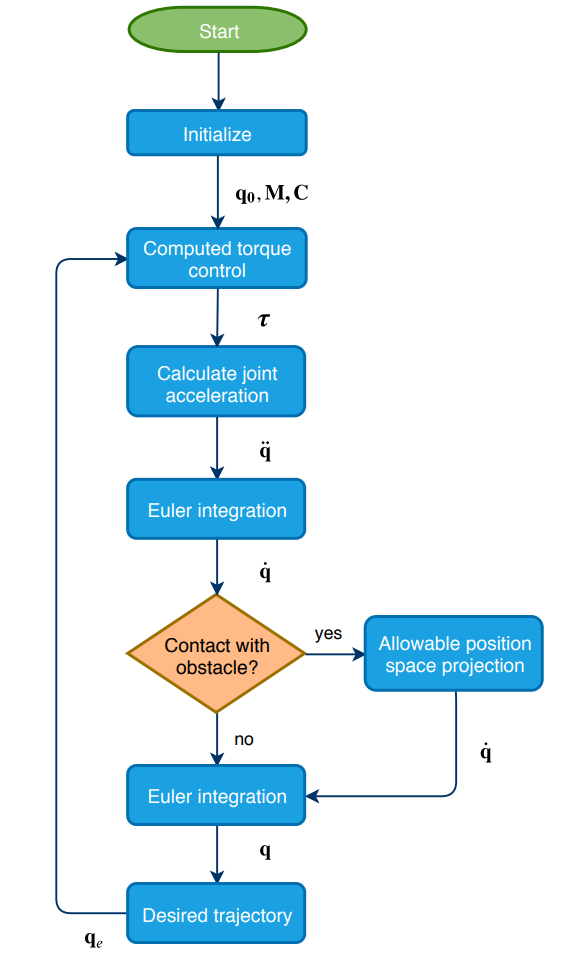
\includegraphics[width=0.75\textwidth]{figures/sysflow.PNG}
    \caption{Program flow diagram}
    \label{fig:prog_flow}
\end{figure}


\section{User guide}

The user can adjust parameters related to the specifications of the snake robot, obstacles in the environment, the desired path the robot should attempt to follow and control parameters. A snapshot of the visual output of these variables are shown in figure \ref{fig:sim_vis}.

\begin{figure}
    \centering
    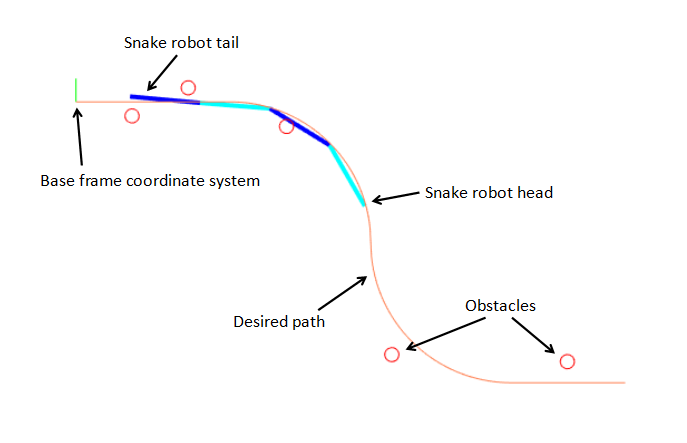
\includegraphics[width=0.9\textwidth]{figures/sim_vis.png}
    \caption{Visual output of simulation}
    \label{fig:sim_vis}
\end{figure}

Once the variables are adjusted in the respective files, the \\ \texttt{initialization.m} script can be run. For a specific configuration, this initialization only has to be run once for every time MATLAB is started. The variables will then end up in the MATLAB workspace and the simulation can be run for a wished number of times. Variables that do not change the dynamics properties of the robot can be redefined without running the whole initialization over.

The user definable variables are summarized in table \ref{tab:sim_userparams}.

\begin{table}
\centering
    \begin{sideways}
    \begin{tabular}{|c|c|c|c|c|}
        \hline
        \textbf{\small{Parameter description}} & \textbf{\small{Parameter name}} & \textbf{\small{Filename}} & \textbf{\small{Datatype}} & \textbf{\small{Unit}}\\
        \hline \hline
        \footnotesize{Number of links} & \texttt{n} & \texttt{init\char`_snake.m} & Integer & \\
        \hline
        \footnotesize{Link length} & \texttt{l}  & \texttt{init\char`_snake.m} & Float & $m$\\
        \hline
        \footnotesize{Link mass} & \texttt{m} & \texttt{init\char`_snake.m} & Float & $kg$\\
        \hline
        \footnotesize{Initial joint angles} & \texttt{q0(1:n)} & \texttt{init\char`_snake.m} & Array of floats & $rad$\\
        \hline
        \footnotesize{Initial position} & \texttt{q0(n+1:n+2)} & \texttt{init\char`_snake.m} & Array of floats & $rad$\\
        \hline
        \footnotesize{Number of obstacles} & \texttt{num\char`_obstacles} & \texttt{init\char`_obstacles.m} & Integer & \\
        \hline
        \footnotesize{Obstacle coordinates} & \texttt{obstacle\char`_coords} & \texttt{init\char`_obstacles.m} & 2D array of floats & $m$\\
        \hline
        \footnotesize{Obstacle safety radius} & \texttt{obstacle\char`_radius} & \texttt{init\char`_obstacles.m} & Float & $m$\\
        \hline
        \footnotesize{Proportional control gain} & \texttt{kp} & \texttt{init\char`_control.m} & Float &\\
        \hline
        \footnotesize{Damping ratio} & \texttt{zeta} & \texttt{init\char`_control.m} & Float &\\
        \hline
        \footnotesize{Torque saturation limit} & \texttt{max\char`_tau} & \texttt{init\char`_control.m} & Float & $Nm$\\
        \hline
        \makecell{\footnotesize{Number of individual }\\\footnotesize{functions defining the path}}  & \texttt{num\char`_sections} & \texttt{init\char`_path.m} & Integer & \\
        \hline
        \makecell{\footnotesize{Intersection point of path}\\\footnotesize{functions along x}}  & \texttt{section\char`_partition} & \texttt{init\char`_path.m} & Array of floats & $m$ \\
        \hline
        \footnotesize{Functions defining the path}  & \texttt{curve} & \texttt{init\char`_path.m} & Set of functions & $m$\\
        \hline
    \end{tabular}
    \end{sideways}
    \caption{User adjustable simulator parameters}
    \label{tab:sim_userparams}
\end{table} 


\section{Program code summary}

The whole simulator is made, and to be executed, in MATLAB. The symbolic toolbox \cite{matlabsymbolic} has been used to generalize the code and make it adaptable to an n-link snake robot. The whole code can be accessed through \hl{...}

The values $l$, $m$, $n$, $N$, $K_p$, $K_d$, $\mathbf{q}$ and $\mathbf{\dot{q}}$ from chapter \ref{chapter:theory} are globally defined and accessible for scripts/functions that might need them.

\subsection{Dynamics functions}

The dynamics, more particularly the matrices $M$ and $C$ from (\ref{eq:eom}), are generated symbolically in the script \texttt{init\char`_dynamics.m}.
As a result of the use of symbols, the matrices can be used as functions with the joint angles and velocities as input parameters.


\subsection{Kinematics functions}\label{subseq:kinfunc}

The script \texttt{init\char`_kinematics.m} generates the transformation matrices from (\ref{eq:transformationmatrix}), defining the relation from base to every link endpoint. These matrices are -- equivalent to the dynamic matrices from last section -- expressed with symbols. Additionally, functions for generating the rotation matrix around the z-axis, \texttt{Rz\char`_func(theta)}, and translation matrix in the x- and y direction, \texttt{D\char`_func(x\char`_dist, y\char`_dist)} are defined.

%-----------------------------------------------------------------------------------------
%-----------------------------------------------------------------------------------------

\subsection{Contact Jacobian function}\label{subseq:Jcfunc}
The symbolic expression of the contact Jacobians is calculated in \\ \texttt{init\char`_contact\char`_jacobians.m}. As there can be a maximum of one obstacle touching each link, there is one general contact Jacobian calculated per link.

\begin{itemize}
    \item \textbf{Lines 2-8:} The position of the contact point in the base frame expressed by the joint variables is extracted from the homogeneous transformation matrix (see section \ref{sec:kin}).
    \item\textbf{Lines 9-12:} Partial differentiation of the position of the contact point with respect to the generalized coordinates to obtain the contact Jacobian.
    \item \textbf{Line 14:} All contact Jacobians are stacked in a 3-dimensional matrix.
\end{itemize}

The variable \texttt{q} represents the vector of generalized coordinates, and \\ \texttt{Rz\char`_func(theta)} and \texttt{D\char`_func(x\char`_dist, y\char`_dist)} are previously defined functions, see \ref{subseq:kinfunc}.

\lstinputlisting[firstline=23, lastline=37]{Simulator_code/init_contact_jacobians.m}

%-----------------------------------------------------------------------------------------
%-----------------------------------------------------------------------------------------

\subsection{Projection function}

The projections are calculated in the function \texttt{calc\char`_projections.m} based on the functions for the contact Jacobians. 

In the following code snippet from the function, contact on link \texttt{i} is already established and the corresponding projection matrices are to be found.

\begin{itemize}
    \item \textbf{Line 2:} The variable \texttt{q(n+2+i,k)} corresponds to the generalized coordinate $d_{c,i}$ (see (\ref{eq:q2})).
    \item \textbf{Lines 3-4:} The contact Jacobian with current $\mathbf{q}$-values from simulation. The function used is explained in \ref{subseq:Jcfunc}.
    \item \textbf{Lines 5-6:} Projection matrices from (\ref{eq:proj_mtrices}).
    \item \textbf{Lines 7-8:} Projection matrices are stacked.
\end{itemize}


\lstinputlisting[firstline=73, lastline=80]{Simulator_code/calc_projections2.m}

Seeing as there might be more than one contact point, several projection matrices are calculated. These matrices are combined by taking the union and intersect as described in \ref{subseq:HPFC}. The logic of the union- and intersect functions are borrowed from Øyvind Stavdahl and presented below.

\lstinputlisting[firstline=89, lastline=97]{Simulator_code/calc_projections2.m}

%-----------------------------------------------------------------------------------------
%-----------------------------------------------------------------------------------------

\subsection{Control}
The following function calculates the joint torques from the computed torque control scheme in \ref{subsec:comp_torque}.

\begin{itemize}
    \item \textbf{Line 3:} See (\ref{eq:controllaw}).
    \item \textbf{Line 5:} Saturation based on the user-adjustable parameter \texttt{max\char`_tau}.
\end{itemize}

\lstinputlisting[]{Simulator_code/computed_torque_control.m}

\subsection{Visualization}

The robot simulation is performed by displaying a figure in which the robot links are redrawn for every time step based on the given robot data. The function in \texttt{visualize.m} takes care of this operation.
\chapter{Experiments} % Results

This chapter presents simulation scenarios chosen to demonstrate the performance and limitations of the simulator, and to show the concept of OAL.

A common configuration for all experiments is given in table \ref{tab:var-allcases}. The individual configurations are presented in the respective sections.

\begin{table}
\centering
    \begin{tabular}{|c|c|c|}
        \hline
         \textbf{Description} & \textbf{Variable name} & \textbf{Value} \\
         \hline
         Link length $[m]$& \texttt{l} & $1$ \\
         \hline
         Link mass $[kg]$& \texttt{m} & $1$ \\
         \hline
         Obstacle safety radius $[m]$& \texttt{obstacle\char`_radius} & $0.1$\\
         \hline
    \end{tabular}
    \caption{Common simulation configuration for all cases}
    \label{tab:var-allcases}
\end{table}



%---------------------------------------------------------------------------------------
%---------------------------------------------------------------------------------------
%---------------------------------------------------------------------------------------

\section{Obstacle-free environment}

This section briefly demonstrates how the robot behaves without the influence of obstacles in the environment.

\subsection{Case 1.1: Single reference computed torque control}

This case is to demonstrate two damping modes of the computed torque controller in a simple scenario. The configurations for the experiment are summarized in table \ref{tab:var-case-1-1}.

\begin{table}
\centering
    \begin{tabular}{|c|c|c|}
        \hline
         \textbf{Description} & \textbf{Variable name} & \textbf{Value} \\
         \hline
         Simulation time $[s]$& \texttt{simTime} & $30$ \\
         \hline
         Simulation sample time $[s]$& \texttt{h} & $0.01$ \\
         \hline
         Number of links & \texttt{n} & $4$ \\
         \hline
         Joint angle setpoints $[rad]$ & \texttt{q\char`_ref} & $[0, \pi/2, -\pi/3, -\pi/2]$ \\
         \hline
         Initial joint angles $[rad]$ & \texttt{q\char`_0(1:n)} & $[0, 0, 0, 0]$ \\
         \hline
         Initial position $[m]$ & \texttt{q\char`_0(n+1:n+2)} & $[0, 0]$ \\
         \hline
    \end{tabular}
    \caption{Simulation configuration for case 1.1}
    \label{tab:var-case-1-1}
\end{table}


Figure \ref{fig:case1-1} shows the different damping-cases using the computed torque controller for following joint angle references. These references are plotted as dashed lines. Please note that the joint angle $q_1 = \phi_1$ is not included as it is a virtual coordinate and not directly actuated.

The critically damped configuration with $\zeta = 1$ is mainly used throughout the experiments. The overdamped case with $\zeta=2$ is used only when very slow motions is desired to avoid abrupt movement. The underdamped case is not relevant for this project and left out.

The proportional gain is chosen to be $\mathbf{K_p} = 0.4 \mathbf{I}$ in all cases. The relation in (\ref{eq:control2}) with $\zeta=1$ and $\zeta=2$ yields $\mathbf{K_d} = 1.3 \mathbf{I}$ and $\mathbf{K_d} = 2.5 \mathbf{I}$ respectively.

\begin{figure}
    \centering

    \subfloat[Critically damped]{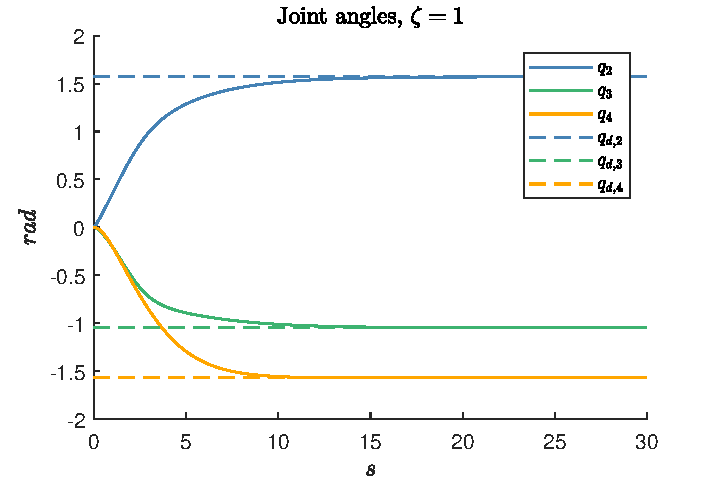
\includegraphics[totalheight=0.4\textheight]{figures/case-1-1/control-critdamped.pdf}}

    \subfloat[Overdamped]{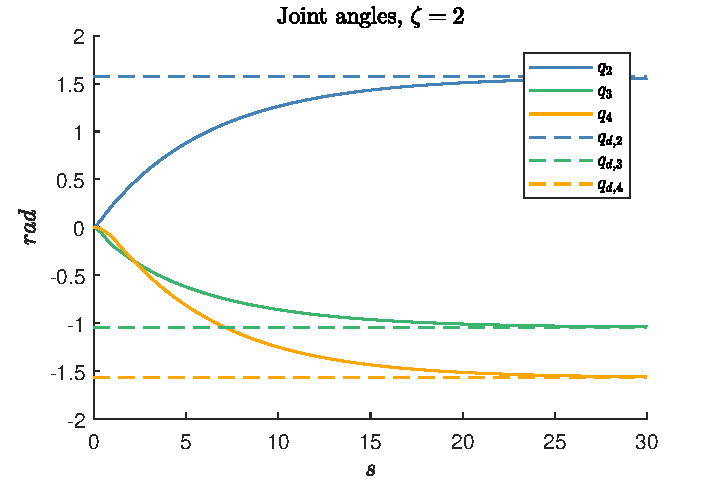
\includegraphics[totalheight=0.4\textheight]{figures/case-1-1/control-overdamped.pdf}}

    \caption{Simulation demo - computed torque control}
    \label{fig:case1-1}
\end{figure}


%---------------------------------------------------------------------------------------
%---------------------------------------------------------------------------------------

\subsection{Case 1.2: Path alignment}\label{subseq:case12}

In this case, the robot is initialized with two different start positions before attempting to adjust to the same path (\ref{eq:path}), which consists of line segments and quadrants. The variable configurations are summarized in table \ref{tab:var-case-1-2}.

The figures \ref{fig:case1-2a} and \ref{fig:case1-2b} show the start and end position of the adjustment in a 15 second interval. It is evident that path adjustment relies on a start configuration close to the path to be successful. However, none of the simulations are able to perfectly adjust to the path. An important reason for this is that the robot cannot change the position of its center of mass without friction or push-points (obstacles) in the environment.

The plots in figure \ref{fig:case1-2-plot} show the joint angles of the controllable joints during the simulations. The reference angles are plotted with a dashed line. It can be observed that he end effector is very close to the path and the corresponding reference angles $q_{d,4}$ are almost met in both cases. Additionally, the reference angles of link 2 and 3 wish to bend the links downward to the path. This is logical, just not completely feasible. A consequence of this is that the robot too far from the path is curling up. The projection method is not considering that the snake robot should be stretched out along the path at all times.

\begin{equation}\label{eq:path}
    y(x) =
    \begin{cases}
        0, & \text{if } x < 2.2 \\
        \sqrt{4 - (x - 2.2)^2} + 2, & \text{if } x \in [2.2, 4.2] \\
        -\sqrt{4 - (x - 6.2)^2} + 2, & \text{if } x \in [4.2, 6.2] \\
        -4, & \text{if } x > 6.2
    \end{cases}
\end{equation}


\begin{table}
\centering
    \begin{tabular}{|c|c|c|}
        \hline
         \textbf{Description} & \textbf{Variable name} & \textbf{Value} \\
         \hline
         Simulation time $[s]$& \texttt{simTime} & $15$ \\
         \hline
         Simulation sample time $[s]$& \texttt{h} & $0.001$ \\
         \hline
         Damping ratio & \texttt{zeta} & $2$ \\
         \hline
         Number of links & \texttt{n} & $4$ \\
         \hline
         Joint angle setpoints $[rad]$ & \texttt{q\char`_ref} & From path \\
         \hline
         Initial joint angles $[rad]$ & \texttt{q\char`_0(1:n)} & $[0, 0, 0, 0]$ \\
         \hline
         \makecell{Initial position part 1 $[m]$\\Initial position part 2 $[m]$} & \texttt{q\char`_0(n+1:n+2)} & \makecell{$[0, 0]$ \\ $[0, -1]$} \\
         \hline
    \end{tabular}
    \caption{Simulation configuration for case 1.2}
    \label{tab:var-case-1-2}
\end{table}


\begin{figure}
    \centering
    
    \subfloat[$t = 0 s$]{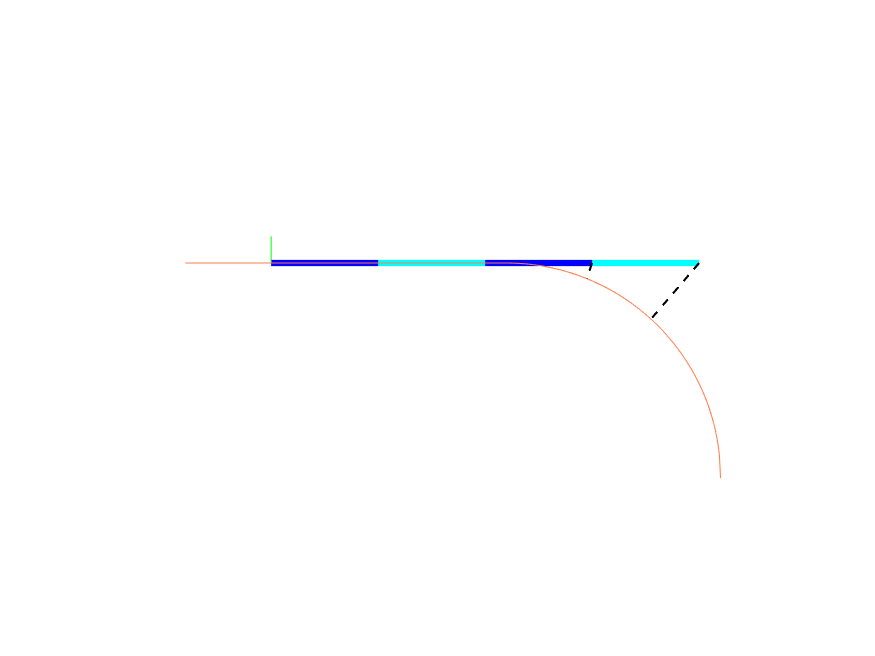
\includegraphics[trim=2cm 2cm 2cm 2cm, clip=true, totalheight=0.23\textheight] {figures/case-1-2/goodgirl1.png}}
    \hfil
    \subfloat[$t = 15 s$]{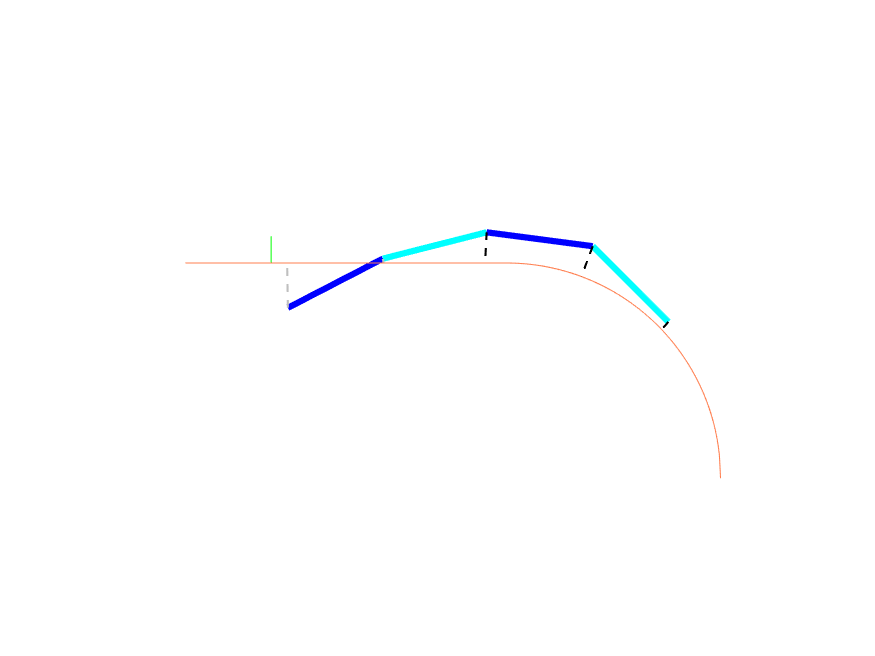
\includegraphics[trim=2cm 2cm 2cm 2cm, clip=true, totalheight=0.23\textheight]{figures/case-1-2/goodgirl3.png}}
    
    \caption{Simulation demo - adjusting to path from nearby}
    \label{fig:case1-2a}
\end{figure}

\begin{figure}
    \centering
    
    \subfloat[$t = 0 s$]{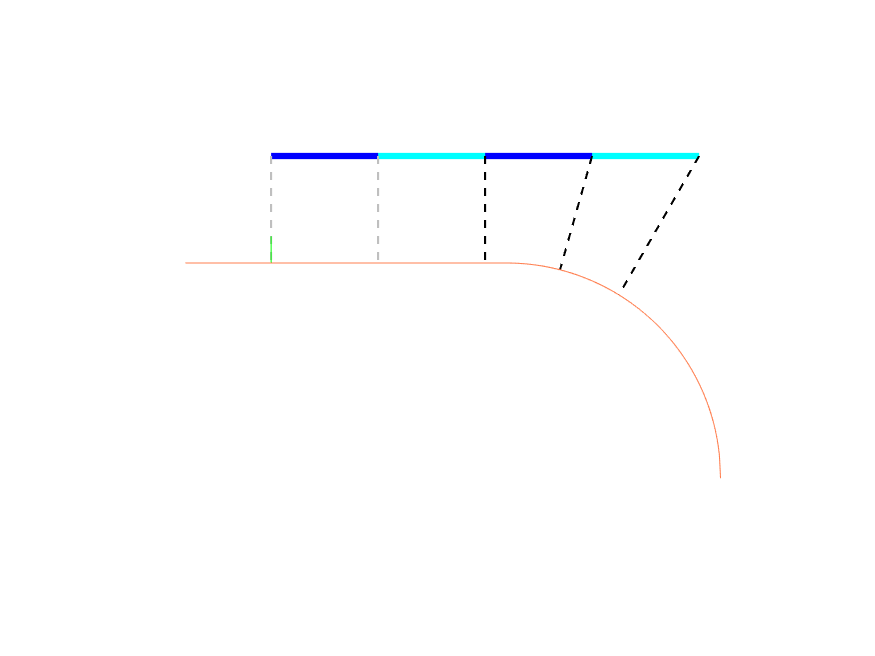
\includegraphics[trim=2cm 2cm 2cm 2cm, clip=true, totalheight=0.23\textheight] {figures/case-1-2/badgirl1.png}}
    \hfil
    \subfloat[$t = 15 s$]{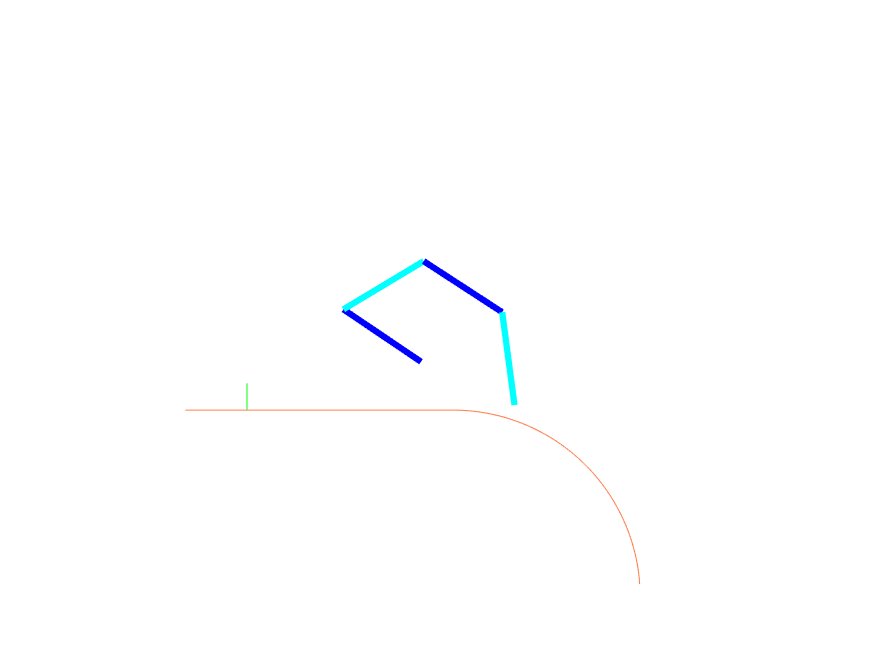
\includegraphics[trim=2cm 2cm 2cm 2cm, clip=true, totalheight=0.23\textheight]{figures/case-1-2/badgirl3.png}}
    
    \caption{Simulation demo - adjusting to path from a distance}
    \label{fig:case1-2b}
\end{figure}

\begin{figure}
    \centering
    
    \subfloat[Start at $(x_0,y_0) = (0,0)$]{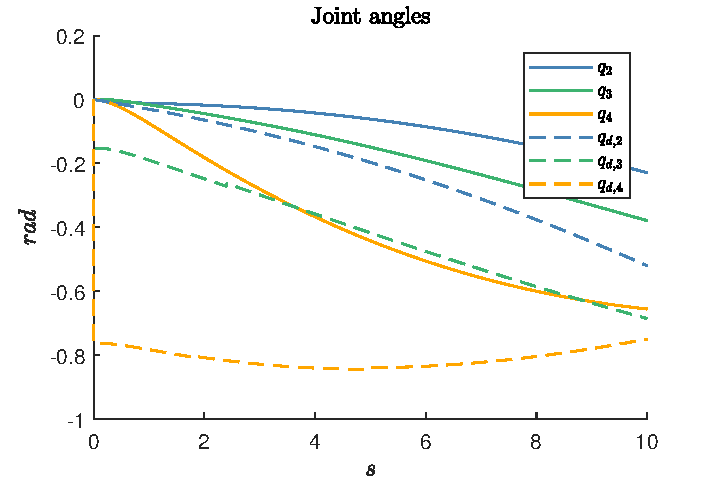
\includegraphics[clip=true, totalheight=0.39\textheight]{figures/case-1-2/case12a.pdf}}

    \subfloat[Start at $(x_0,y_0) = (0,-1)$]{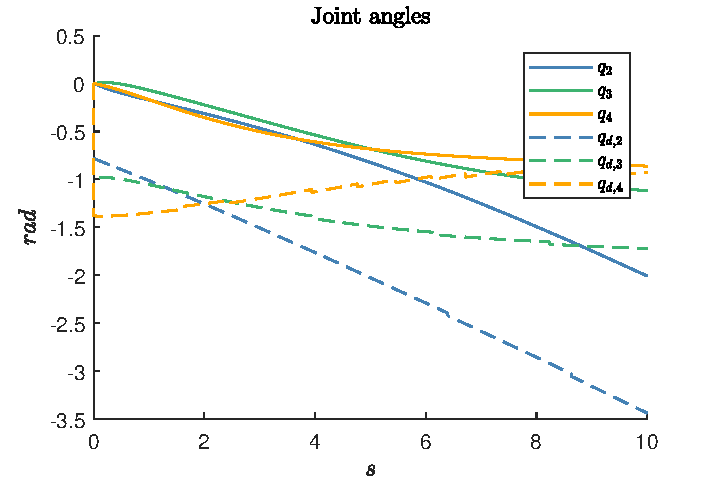
\includegraphics[clip=true, totalheight=0.39\textheight]{figures/case-1-2/case12b.pdf}}

    \caption{Joint angles for path adjustment with different starting configurations}
    \label{fig:case1-2-plot}
\end{figure}

%---------------------------------------------------------------------------------------
%---------------------------------------------------------------------------------------
%---------------------------------------------------------------------------------------

\section{OAL simulation scenarios}

\subsection{Case 2.1: Simple propulsion}\label{subseq:case21}

This scenario aims a demonstrating the concept of OAL. The snake robot is simply set to bend its front joint to $-\pi/2$ while the other joints are to remain in a stretched out configuration. The simulator variable configuration can be seen in table \ref{tab:var-case-2-1}.
\begin{table}
\centering
    \begin{tabular}{|c|c|c|}
        \hline
         \textbf{Description} & \textbf{Variable name} & \textbf{Value} \\
         \hline
         Simulation time $[s]$& \texttt{simTime} & $20$ \\
         \hline
         Simulation sample time $[s]$& \texttt{h} & $0.001$ \\
         \hline
         Damping ratio & \texttt{zeta} & $2$ \\
         \hline
         Number of links & \texttt{n} & $4$ \\
         \hline
         Joint angle setpoints $[rad]$ & \texttt{q\char`_ref} & $[0, 0, 0, -\pi/2]$ \\
         \hline
         Initial joint angles $[rad]$ & \texttt{q\char`_0} & $[0, 0, 0, 0]$ \\
         \hline
         Number of obstacles & \texttt{num\char`_obstacles} & $3$ \\         
         \hline
         Obstacle positions $[m]$& \texttt{obstacle\char`_coords} & \makecell{$(0.8, -0.08)$ \\ $(1.6, 0.08)$ \\ $(3.3, -0.3)$} \\
         \hline
    \end{tabular}
    \caption{Simulation configuration for case 2.1}
    \label{tab:var-case-2-1}
\end{table}

The setpoints are manually set based on the knowledge that the bending link will collide with an obstacle in trying to fulfill the task. In order to obtain the desired angle, the link will apply a force to the obstacle underneath and consequently drag the whole robot body in the positive $x$ (rightward) direction. A sequence of the movement is presented in figure \ref{fig:case2-1}. The obstacles laying close to the rear links are positioned to allow the rest of the robot to stay flat. From the figure it can be seen that the robot moves away from the obstacles towards the end without pushing against anything. This is a consequence of the modeled frictionless environment.

\begin{figure}
    \centering
    
    \subfloat[$t = 0 s$]{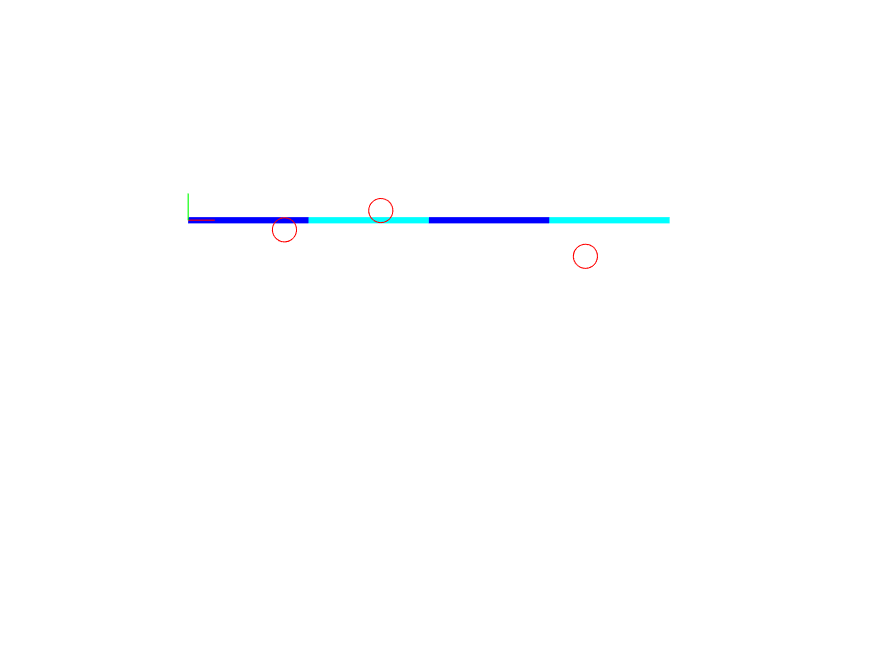
\includegraphics[trim=2cm 4cm 2cm 1.5cm, clip=true, totalheight=0.18\textheight] {figures/case-2-1/sim1.png}}
    \hfil
    \subfloat[$t = 4 s$]{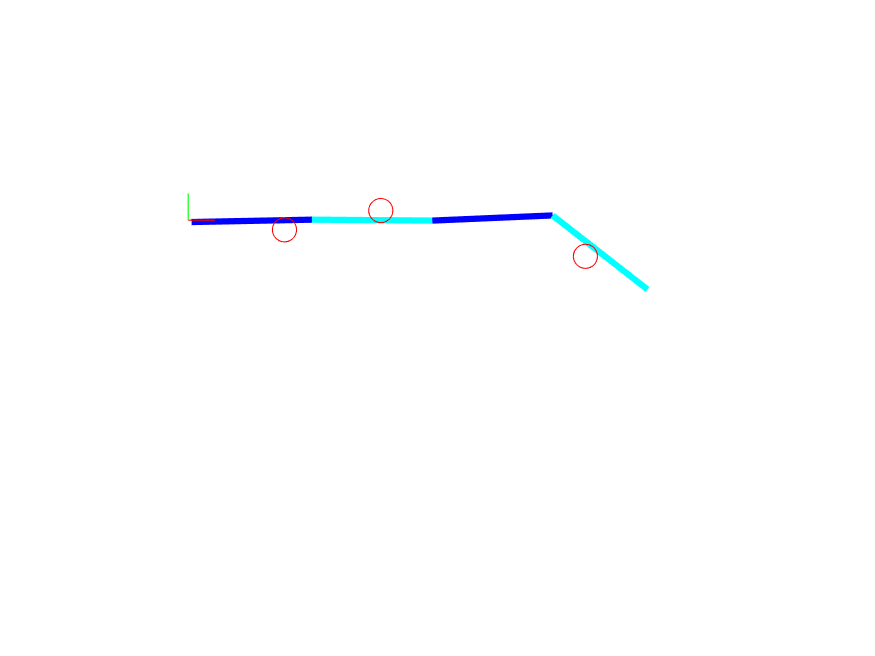
\includegraphics[trim=2cm 4cm 2cm 1.5cm, clip=true, totalheight=0.18\textheight]{figures/case-2-1/sim2.png}}
    
    \subfloat[$t = 8 s$]{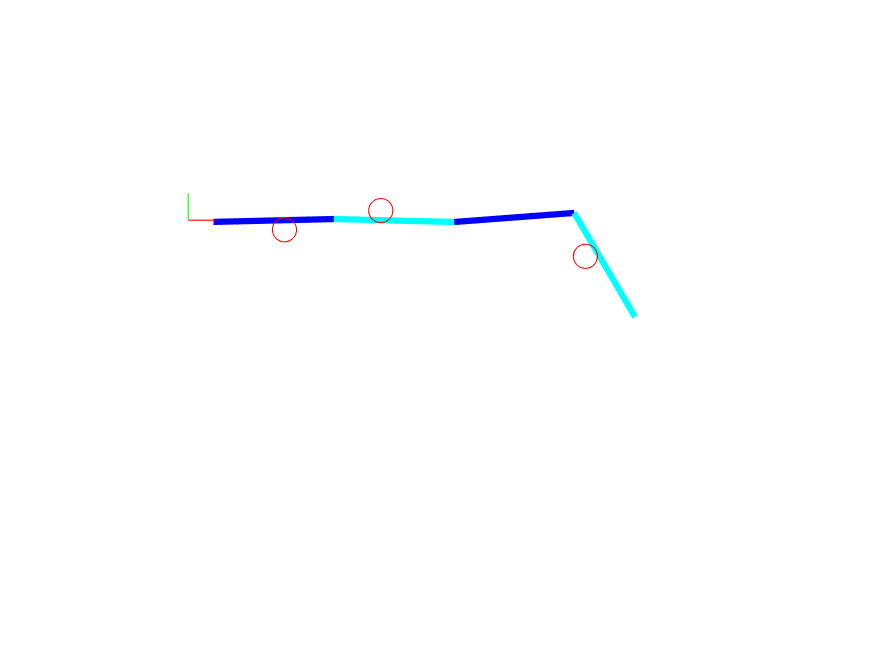
\includegraphics[trim=2cm 4cm 2cm 1.5cm, clip=true, totalheight=0.18\textheight]{figures/case-2-1/sim3.png}}
    \hfil
    \subfloat[$t = 12 s$]{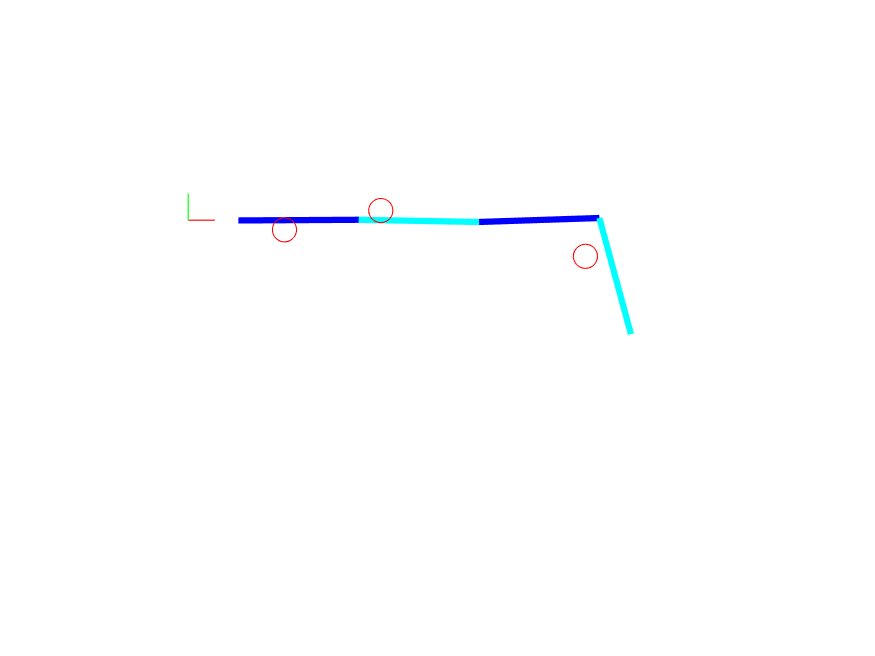
\includegraphics[trim=2cm 4cm 2cm 1.5cm, clip=true, totalheight=0.18\textheight]{figures/case-2-1/sim4.png}}

    \subfloat[$t = 16 s$]{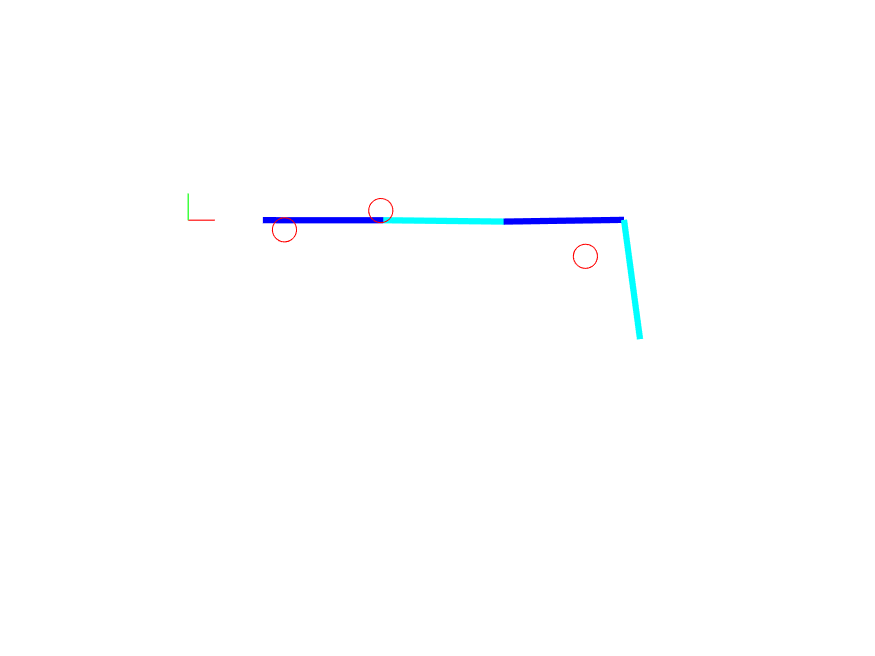
\includegraphics[trim=2cm 4cm 2cm 1.5cm, clip=true, totalheight=0.18\textheight]{figures/case-2-1/sim5.png}}
    \hfil
    \subfloat[$t = 20 s$]{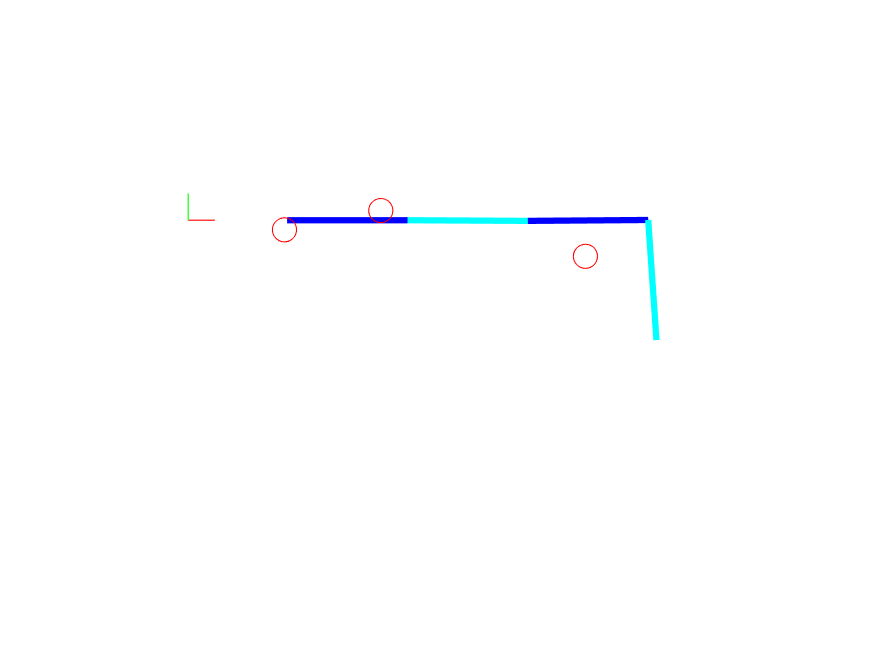
\includegraphics[trim=2cm 4cm 2cm 1.5cm, clip=true, totalheight=0.18\textheight]{figures/case-2-1/sim6.png}}

    \caption{Simulation demo - propulsion with static joint setpoint}
    \label{fig:case2-1}
\end{figure}

From the plots in figure \ref{fig:case2-1-plot} it is clear that the collision with the lower obstacle takes place at \textasciitilde{} 3 seconds. At this point, the joint velocities are projected such that the front link moves to the edge of the obstacle. Additionally, the preceding joints experience an offset as the front joint applies a torque that influences the whole robot.

A repercussion of the geometrical approximation of the contact forces becomes obvious in this experiment. The joint velocities in the emphasised time span in part (b) of figure \ref{fig:case2-1-plot} admit a twitching behaviour as a result of the velocity projections. This circumstance is discussed in chapter \ref{ch:discussion}.

\begin{figure}
    \centering
    
    \subfloat[]{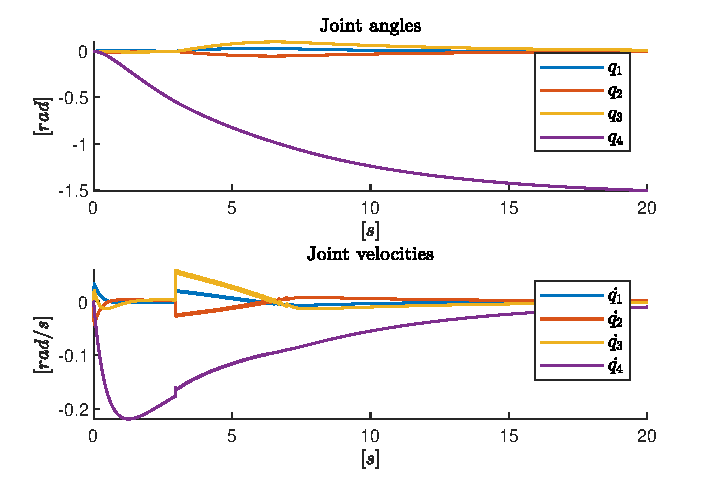
\includegraphics[clip=true, totalheight=0.39\textheight]{figures/case-2-1/case21.pdf}}

    \subfloat[Zoom of joint velocities in seconds 5-10]{\fbox{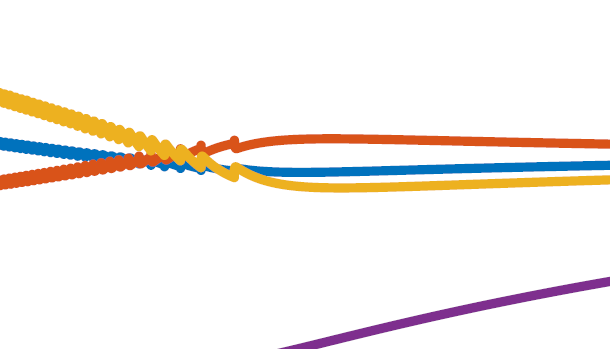
\includegraphics[clip=true, totalheight=0.18\textheight]{figures/case-2-1/zoom21.PNG}}}

    \caption{Joint- angles and velocities for the single setpoint scenario}
    \label{fig:case2-1-plot}
\end{figure}

%---------------------------------------------------------------------------------------
%---------------------------------------------------------------------------------------

\subsection{Case 2.2: No propulsion}\label{subseq:case22}

As propulsion requires a force in the respective direction, there are scenarios where a set of joint torques are insufficient for attaining this force. This scenario aims at illustrating the case where the forces applied work against each other in the direction of propulsion and the robot is simply deformed. The variable configuration for the simulation is presented in table \ref{tab:var-case-2-2} and figure \ref{fig:case2-2} shows a sequence of the motion.

\begin{table}
\centering
    \begin{tabular}{|c|c|c|}
        \hline
         \textbf{Description} & \textbf{Variable name} & \textbf{Value} \\
         \hline
         Simulation time $[s]$& \texttt{simTime} & $9$ \\
         \hline
         Simulation sample time $[s]$ & \texttt{h} & $0.001$ \\
         \hline
         Damping ratio & \texttt{zeta} & $1$ \\
         \hline
         Number of links & \texttt{n} & $3$ \\
         \hline
         Joint angle setpoints $[rad]$& \texttt{q\char`_ref} & $[0, -\pi/3, \pi/3]$ \\
         \hline
         Initial joint angles $[rad]$& \texttt{q\char`_0} & $[0, 0, 0]$ \\
         \hline
         Number of obstacles & \texttt{num\char`_obstacles} & $3$ \\         
         \hline
         Obstacle positions $[m]$& \texttt{obstacle\char`_coords} & \makecell{$(0.5, 0.1)$ \\ $(1.5, -0.1)$ \\ $(2.5, 0.1)$} \\
         \hline
    \end{tabular}
    \caption{Simulation configuration for case 2.2}
    \label{tab:var-case-2-2}
\end{table}


\begin{figure}
    \centering
    
    \subfloat[$t = 0 s$]{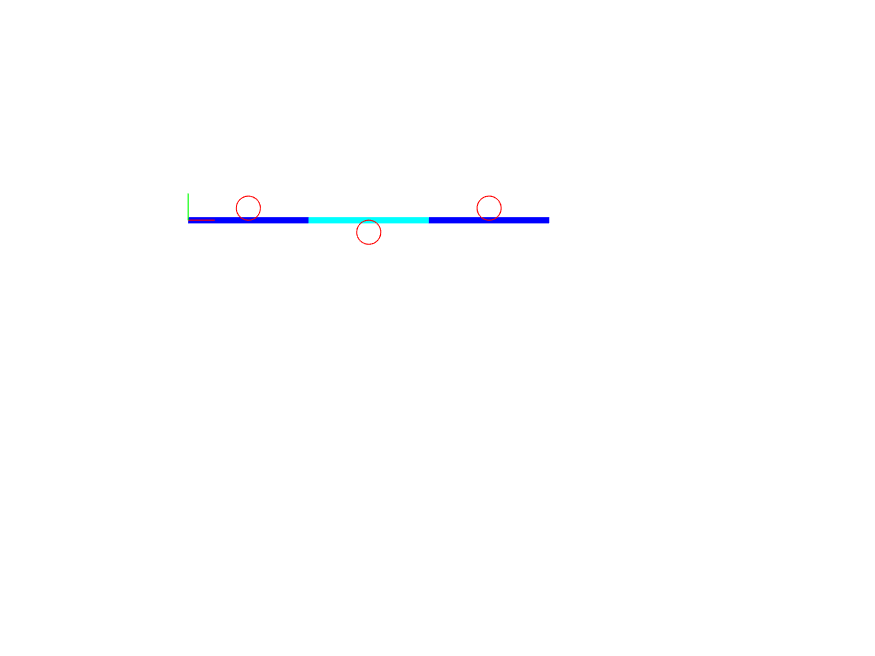
\includegraphics[trim=2cm 4cm 2cm 1.5cm, clip=true, totalheight=0.18\textheight] {figures/case-2-2/2sim1.png}}
    \hfil
    \subfloat[$t = 3 s$]{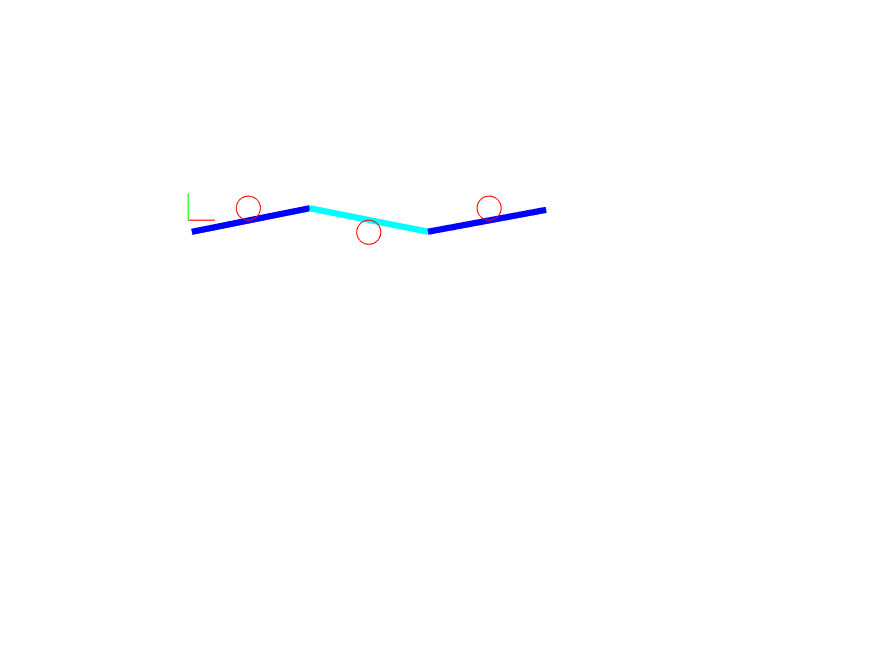
\includegraphics[trim=2cm 4cm 2cm 1.5cm, clip=true, totalheight=0.18\textheight]{figures/case-2-2/2sim2.png}}
    
    \subfloat[$t = 6 s$]{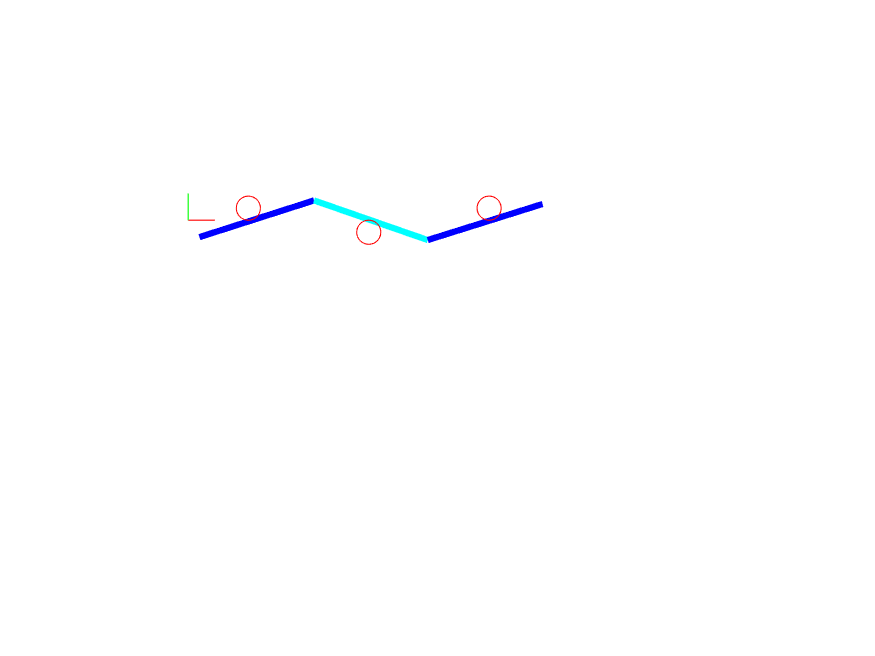
\includegraphics[trim=2cm 4cm 2cm 1.5cm, clip=true, totalheight=0.18\textheight]{figures/case-2-2/2sim3.png}}
    \hfil
    \subfloat[$t = 9 s$]{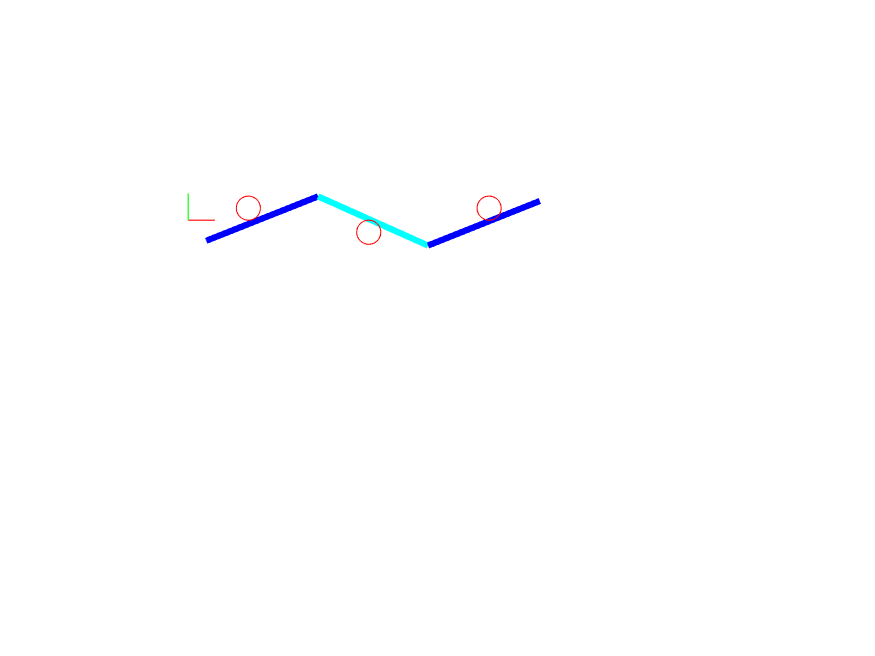
\includegraphics[trim=2cm 4cm 2cm 1.5cm, clip=true, totalheight=0.18\textheight]{figures/case-2-2/2sim4.png}}
    
    \caption{Simulation demo - no propulsion}
    \label{fig:case2-2}
\end{figure}

%---------------------------------------------------------------------------------------
%---------------------------------------------------------------------------------------

\subsection{Case 2.3: Propulsion along path}\label{subseq:case23}

This case is to illustrate how the robot can aid obstacles to propel along a defined path. Since the robot is only position controlled based on deviation from the path, the obstacles are placed in a manner that supports both the desired shape and motion. This configuration can be seen in figure \ref{}. The two obstacles in the back are to keep the rear links on the path, while the obstacle in front is placed so that the robot can push against it and pull itself forward. In order for this to happen, the obstacle has been placed slightly on the path, leading to a constant error from the path. The robot's desire to always stay as close to the path as possible makes it push against the obstacle.

The variable configurations are presented in table \ref{tab:var-case-2-3}. The desired path (\ref{eq:path}) is the same one as in \ref{subseq:case12}.


\begin{table}
\centering
    \begin{tabular}{|c|c|c|}
        \hline
         \textbf{Description} & \textbf{Variable name} & \textbf{Value} \\
         \hline
         Simulation time $[s]$ & \texttt{simTime} & $240$ \\
         \hline
         Simulation sample time $[s]$ & \texttt{h} & $0.001$ \\
         \hline
         Damping ratio & \texttt{zeta} & $1$ \\
         \hline
         Number of links & \texttt{n} & $5$ \\
         \hline
         Joint angle setpoints $[rad]$& \texttt{q\char`_ref} & From path \\
         \hline
         Initial joint angles $[rad]$ & \texttt{q\char`_0} & $[0, 0, 0, 0, 0]$ \\
         \hline
         Number of obstacles & \texttt{num\char`_obstacles} & $3$ \\         
         \hline
         Obstacle positions $[m]$& \texttt{obstacle\char`_coords} & \makecell{$(0.8, -0.1)$ \\ $(1.6, 0.1)$ \\ $(3.2, -0.35)$} \\
         \hline
    \end{tabular}
    \caption{Simulation configuration for case 2.3}
    \label{tab:var-case-2-3}
\end{table}

The movement, as well as the desired path (red), is shown in figure \ref{fig:case2-3}. It is clear that when the robot loses contact with the environment (at approximately 200 seconds), it has trouble with staying close to the path. Keep in mind that all movement is frictionless and that the robot therefore may keep on moving in a direction without simultaneously applying a force to the environment.

Robot moving slightly through obstacle radius towards the end.

\begin{figure}
    \centering
    
    \subfloat[$t = 0 s$]{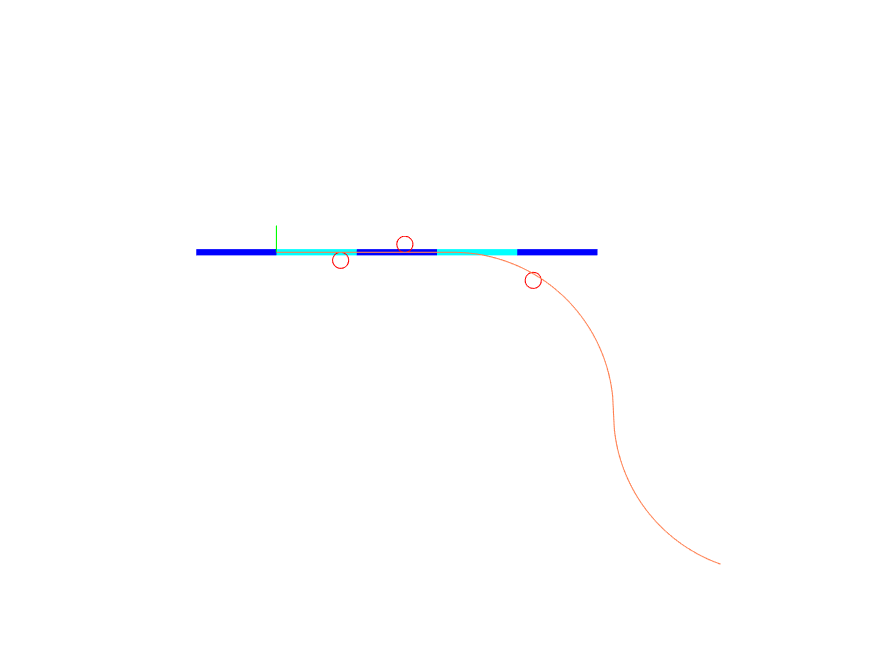
\includegraphics[trim=2cm 3cm 2cm 3cm, clip=true, totalheight=0.15\textheight] {figures/case-2-3/sim1.png}}
    \hfil
    \subfloat[$t = 40 s$]{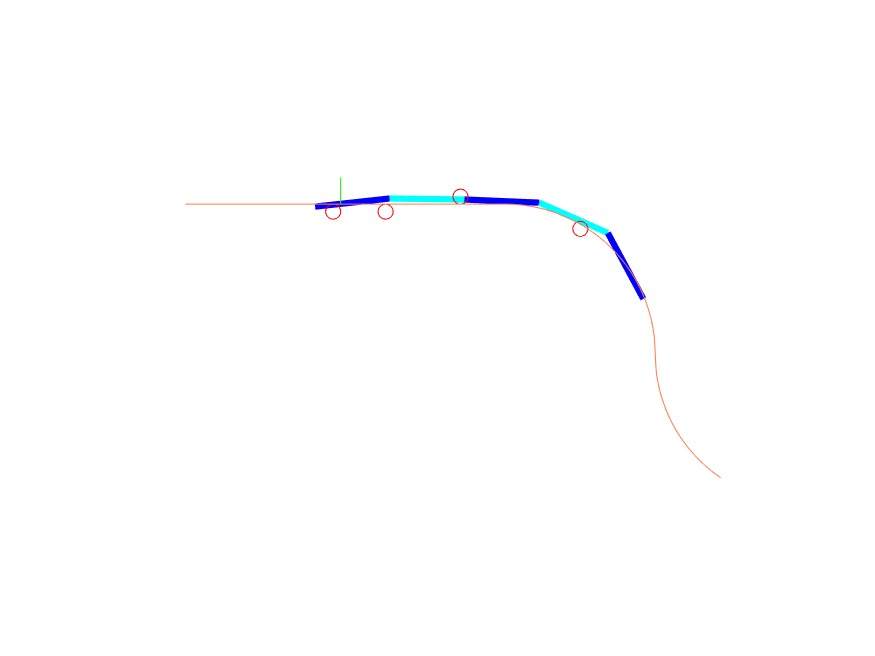
\includegraphics[trim=2cm 3cm 2cm 3cm, clip=true, totalheight=0.15\textheight]{figures/case-2-3/sim3.png}}
    
    \subfloat[$t = 80 s$]{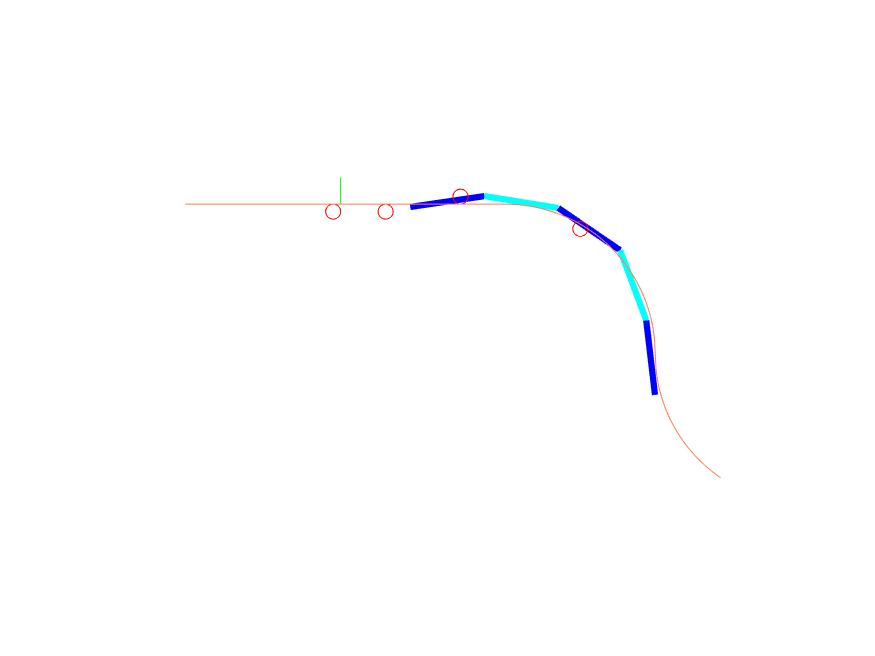
\includegraphics[trim=2cm 3cm 2cm 3cm, clip=true, totalheight=0.15\textheight]{figures/case-2-3/sim5.png}}
    \hfil
    \subfloat[$t = 120 s$]{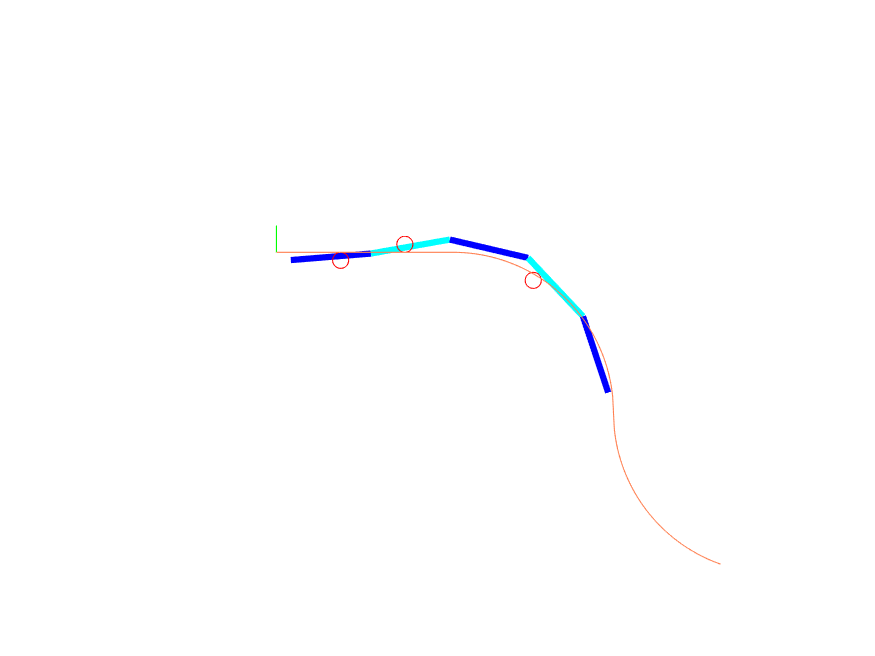
\includegraphics[trim=2cm 3cm 2cm 3cm, clip=true, totalheight=0.15\textheight]{figures/case-2-3/sim7.png}}

    \subfloat[$t = 160 s$]{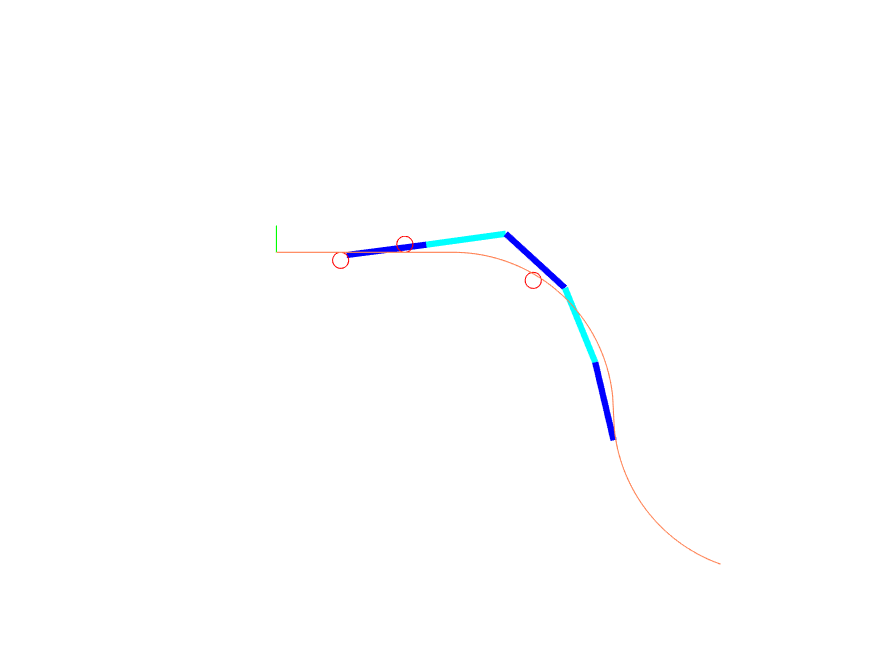
\includegraphics[trim=2cm 3cm 2cm 3cm, clip=true, totalheight=0.15\textheight]{figures/case-2-3/sim9.png}}
    \hfil
    \subfloat[$t = 200 s$]{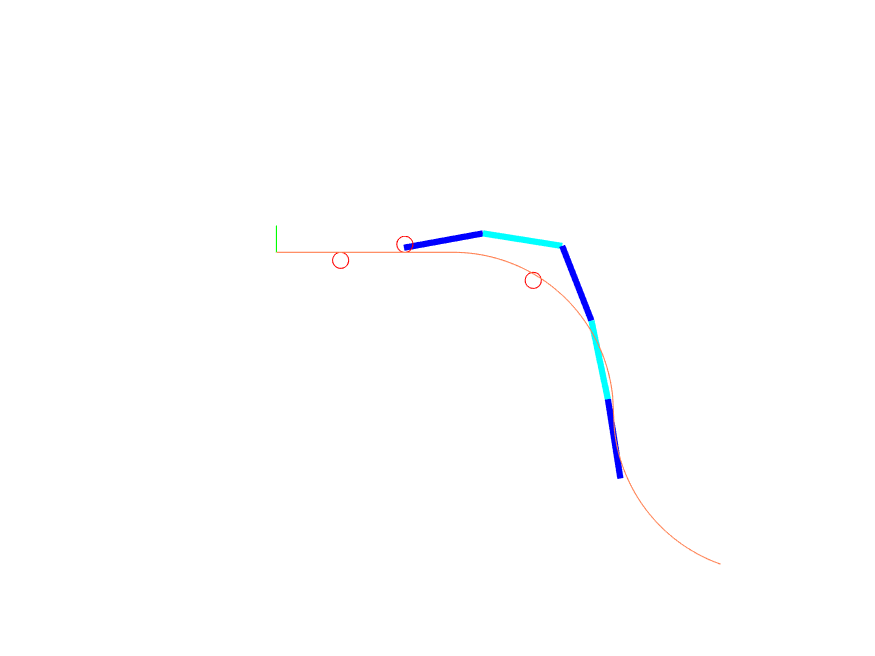
\includegraphics[trim=2cm 3cm 2cm 3cm, clip=true, totalheight=0.15\textheight]{figures/case-2-3/sim92.png}}
    
    \subfloat[$t = 220 s$]{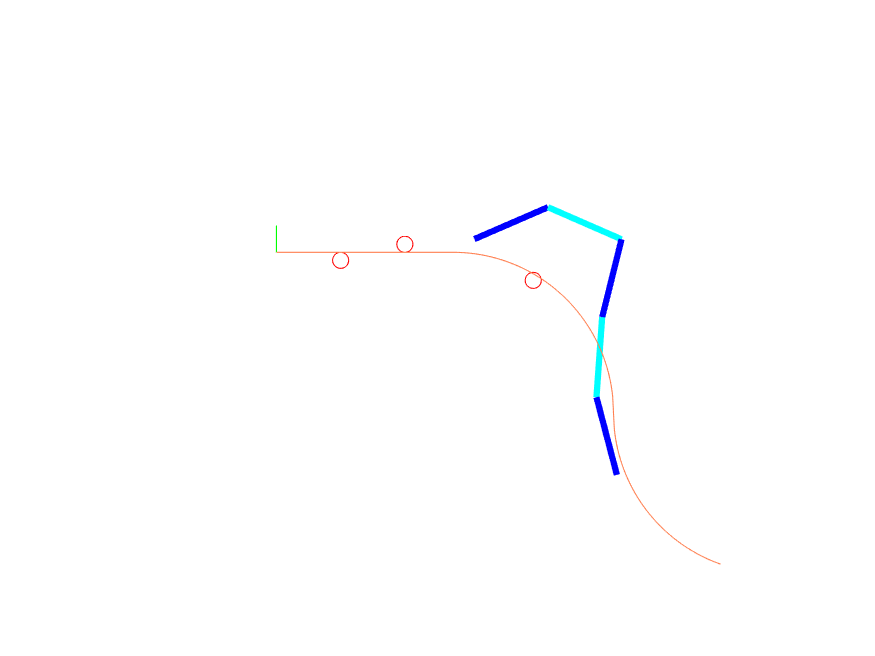
\includegraphics[trim=2cm 3cm 2cm 3cm, clip=true, totalheight=0.15\textheight]{figures/case-2-3/sim94.png}}
    \hfil

    \caption{Simulation demo - propulsion along path}
    \label{fig:case2-3}
\end{figure}

%---------------------------------------------------------------------------------------
%---------------------------------------------------------------------------------------

\subsection{Case 2.4: Unsuccessful propulsion attempt along path}
Robot går baklengst.
Vis sekvens. Plot av posisjon til hodet og path.
Kanskje det funker på samme scenario som simple propulsion, bare med hindringene på andre posisjoner.

%---------------------------------------------------------------------------------------
%---------------------------------------------------------------------------------------
%---------------------------------------------------------------------------------------


\chapter{Discussion} \label{ch:discussion}

This chapter looks at the effects of simplifications and approximations made during the development of the simulator both in regard of the dynamical model and in regard of the path following method. These effects, as well as the general results from the experiments are discussed and some improvements are proposed.

\section{Effects of the contact behaviour simplification}

The geometrical approximation made regarding the contact forces between the robot and the obstacles have been characteristic for the outcome of the simulations. Firstly, it might not yield unique solutions, leading to unpredictable or unrealistic behavior in some scenarios. Secondly, it has been observed that the robot in some cases ends up moving slightly over the edge of obstacles when there are several "conflicting" constraints present.

From a physical perspective, it is obvious that projecting the velocities to an "allowable space" just based on the positioning of the obstacles differs from the resulting velocities after a collision. Projecting the velocities means that the velocity of the robot body might be increased after contact with an obstacle. This does in turn mean increasing the total energy of the system, which contradicts basic laws of physics.  

There are of course several methods that could have avoided this simplification.
One option would be to implicitly define the forces as a part of the dynamical model, in the same way as the forces between the joints in the robot are implicitly defined. The method of Yoshikawa \cite{yoshikawa1987dynamic}, explained in \ref{subseq:dynhpfc}, follows this approach. It does however only consider constraints on the end effector of the robot, and not on arbitrary links. The adjustment that has to be made in the snake robot case, is that the constraint hypersurfaces and forces onto these surfaces have to be defined for every contact point.

%\hl{Could we have used Paf to find the component belonging to the constraint++ space???}

Another consequence of the geometrical approximation, is that the projection matrices only allow movement along obstacles. This is necessary for preventing the robot in moving through obstacles, but also prevents the robot from perpendicularly moving away from them. In other words, whenever a link comes in contact with an obstacle, it will stick to it until it has slid along it. This strict positioning of the links can come in conflict with the controller and path projection. The only case in which a link "detaches" from the obstacle before sliding all the way along it, is when it in a discrete time step is projected to a position where it no longer is considered in contact and fazed by the obstacle.

Yet another important remark, is that the program treats the cases in which a link is on the edge of the obstacle radius and within the obstacle radius equally. In particular, it considers both cases a point contact and disregards how close it is to the actual obstacle point. In \ref{subseq:case23} it is pointed out that the robot slides slightly through this radius, but keep in mind that for the robot it is the same as sliding on the edge. However, it is of course a mistake that the robot ended up within the radius in the first place, but it is most probably a result of the discrete nature of the simulator. Furthermore, it is the velocity rather than position of the robot that is changed with the projection. The robot might thus still be inside the obstacle radius at the next time step. Decreasing the radius would naturally also decrease this effect, but it is still crucial to keep in the discrete simulations.

A workaround for the rigid definition of contact, in which the robot is either completely in contact with the obstacle or not at all, could be introducing an elastic radius or force field around the obstacles, and thus damp the nonlinear effects of the interactions. %PD controller


\section{Review of the path alignment method}

The method of finding the desired angles based on projection onto the path is not robust in cases where the links are far from the path (see experiment in \ref{subseq:case12}). The simplest solution would be avoiding the projection of links that are very misplaced. A future, more advanced, solution would be redefining the optimal path to overlap with the current position of the robot. In \ref{subseq:case12} it is pointed out that the method of finding the desired joint angles disregards the positions of the two first joints, or rather the position of the start- and end point of the tail-link. Correcting this poor quality would improve the performance of the path following capability significantly. Situations like in \ref{subseq:case24} where the tail of the robot gets stuck would then be avoided.

The desired joint angles from the path projection method are calculated separately for each link in the current program. A more robust and intelligent solution would be defining an objective function that considers the deviation from the path for all joints, and then finds the set of joint desired angles minimizing the complete set of deviations. By this method it would also be possible to weight the error of the snake robot head the most. Holden \cite{holden2014optimal} has formulated an optimization problem that finds input torques by minimizing energy consumption while achieving propulsion along the desired path. The method is a great inspiration, but not quite yet a solution to the problem as it still requires the desired joint angles at the obstacles.

\section{Further insights from experiments}

On the more constructive side, it is clear that the simulator has proven to be a great resource for presenting concepts and study the possibilities within obstacle aided locomotion. Furthermore, the modular architecture of the program, where controller, dynamics, path following etc. is decoupled, allows for it to be effortlessly modified.

The experiments have shown that the positioning of the obstacles and path in relation to each other is vital for the propulsion of the robot. This is especially the case in an environment where the possibility to aid friction for propulsion is absent. Furthermore, it has been shown that it is necessary to have a sufficient number of obstacles. Not only for the propulsion, but also for continuously aiding the robot with alignment along the path. Consequently, a limitation of the implemented system is that the configuration of obstacles and desired path need to be determined manually.

A further observation from the experiments, in particular \ref{subseq:case23}, is that the obstacles used for aligning the rear part of the robot are comparable to a manipulator base. More specifically, the robot is in this position able to keep its rear links fixed in the perpendicular direction and thus control the proceeding links to go in this direction
This does in turn lead to the robot being able to get further with a greater number of links, as the robot slides through the aligning obstacles for a longer period of time.

When it comes to the computational performance of the simulator, it is observed that the program requires significantly more time for computing the initialization of robots with 6 links or more than that of robots with fewer links. An improvement would have been defining the equations of motion directly rather than performing symbolic math differentiation to derive them. However, the initialization only has to run once for every configuration, and the real time visual performance of the actual simulation is still satisfactory for sample times greater than 0.001 seconds.




\chapter{Outlook}\label{outlook}

Future work.
Path planning. Dynamic model of everything / definition/analysis of constraints. 


%\appendix{}
%
\chapter{Figures}
\section{Example 1}
\cmark
\section{Example 2}
\xmark


\printglossaries
\printbibliography{}

\end{document}
